%!TeX root=../document.tex

\chapter{Equations of Motion}

\section{Introduction}

\subsection{Single Element Equation}

Consider a single, unconstrained finite element with index~$k$ and~$n$ degrees of freedom.
Its configuration at time~$t$ will be described by the displacement vector~$\boldsymbol{u}_{k}(t) \in \mathbb{R}^n$ containing all the coordinates of the element's nodes.
For the kinds of elements that we will use, the equation of motion takes the form

\begin{equation}
\boldsymbol{M}_{k}\,\ddot{\boldsymbol{u}}_{k}(t) + \boldsymbol{D}_{k}\,\dot{\boldsymbol{u}}_{k}(t) + \boldsymbol{Q}_{k}(\boldsymbol{u}_{k}(t)) = \boldsymbol{P}_{k}(t).\label{eq:local-equation-of-motion}
\end{equation}

This is a nonlinear ordinary differential equation of second order for the displacements~$\boldsymbol{u}_{k}(t)$.
The matrix ~$\boldsymbol{M}_{k} \in \mathbb{R}^{n \times n}$ is called the element's mass matrix.
It defines the element's inertial forces and is constant and positive definite.
The matrix~$\boldsymbol{D}_{k} \in \mathbb{R}^{n \times n}$ is the element's damping matrix and defines a linear relationship between the velocities~$\dot{\boldsymbol{u}}_{k}(t)$ and the resulting damping forces.
It is also constant and positive semi-definite.
The only nonlinear term in the equation is the vector of elastic forces,~$\boldsymbol{Q}_{k} \in \mathbb{R}^n$, which depends on the displacements in an arbitrary way.

In the following chapters we are going to derive the components of this element equation for the various elements used in VirtualBow, but first let's consider the overall system that results from combining multiple such elements.

\newpage
\subsection{Overall System Equation}

If the overall finite element system has a total of~$N$ degrees of freedom, it's configuration can be described by the global displacement vector~$\boldsymbol{u}(t) \in \mathbb{R}^{N}$.
The local element displacements~$\boldsymbol{u}_{k}$ are now no longer independent but instead directly related to the global displacements of the system they are part of.
In our case these connectivity constraints can be written as

\begin{equation}
\boldsymbol{u}_{k}(t) = \boldsymbol{A}_{k}\,\boldsymbol{u}(t) + \boldsymbol{b}_{k},\label{eq:kinematics-local-global}
\end{equation}

where~$\boldsymbol{A}_{k} \in \mathbb{R}^{\mathlarger{n} \times N}$ describes a linear transformation and~$\boldsymbol{b}_{k} \in \mathbb{R}^{N}$ describes a constant translation or offset for the respective element displacements.
Applying this kinematic relationship to the local equations of motion~(\ref{eq:local-equation-of-motion}) leads to the element equations expressed in the global coordinates~$\boldsymbol{u}(t)$,

\begin{equation}
\boldsymbol{A}_{k}^\intercal\boldsymbol{M}_{k}\boldsymbol{A}_{k}\,\ddot{\boldsymbol{u}}(t) + \boldsymbol{A}_{k}^\intercal\boldsymbol{D}_{k}\,\boldsymbol{A}_{k}\,\dot{\boldsymbol{u}}(t) + \boldsymbol{A}_{k}^\intercal\boldsymbol{Q}_{k}(\boldsymbol{A}_{k}\,\boldsymbol{u}(t) + \boldsymbol{b}_{k}) = \boldsymbol{A}_{k}^\intercal\boldsymbol{P}_{k}.
\end{equation}

And finally, by summing up the element contributions, the equation of motion of the overall system turns out to have the same structure as the element equations,

\begin{equation}
\boldsymbol{M}\,\ddot{\boldsymbol{u}} + \boldsymbol{D}\,\dot{\boldsymbol{u}} + \boldsymbol{Q}(\boldsymbol{u}) = \boldsymbol{P}(t)\label{eq:global-equation-of-motion}
\end{equation}

where the global mass matrix $\boldsymbol{M} \in \mathbb{R}^{N \times N}$, damping matrix $\boldsymbol{D} \in \mathbb{R}^{N \times N}$, internal forces~$\boldsymbol{Q} \in \mathbb{R}^{N}$ and external forces $\boldsymbol{P} \in \mathbb{R}^{N}$ are calculated from the local element matrices as

\begin{align}
\boldsymbol{M} &= \sum_{k} \boldsymbol{A}_{k}^\intercal\boldsymbol{M}_{k}\boldsymbol{A}_{k} \\
\boldsymbol{D} &= \sum_{k} \boldsymbol{A}_{k}^\intercal\boldsymbol{D}_{k}\boldsymbol{A}_{k} \\
\boldsymbol{Q} &= \sum_{k} \boldsymbol{A}_{k}^\intercal\boldsymbol{Q}_{k}(\boldsymbol{A}_{k}\,\boldsymbol{u} + \boldsymbol{b}_{k}) \\
\boldsymbol{P} &= \sum_{k} \boldsymbol{A}_{k}^\intercal\boldsymbol{P}_{k}
\end{align}

In order to solve the equations of motion for equilibrium we're later going to need the derivative of the elastic forces with respect to the displacements, which is called the tangent stiffness matrix~$\boldsymbol{K} \in \mathbb{R}^{N \times N}$ of the system and can be calculated from the element's local tangent stiffness matrices~$\boldsymbol{K}_{k} = \partial \boldsymbol{Q}_{k} / \partial \boldsymbol{u}_{k}$ as

\begin{align}
\boldsymbol{K}(\boldsymbol{u}) &= \frac{\partial \boldsymbol{Q}}{\partial \boldsymbol{u}} = \frac{\partial}{\partial \boldsymbol{u}} \sum_{k} \boldsymbol{A}_{k}^\intercal\boldsymbol{Q}_{k}(\boldsymbol{A}_{k}\,\boldsymbol{u} + \boldsymbol{b}_{k}) \notag \\
&= \sum_{k} \boldsymbol{A}_{k}^\intercal \frac{\partial}{\partial \boldsymbol{u}_{k}}\boldsymbol{Q}_{k}(\boldsymbol{A}_{k}\,\boldsymbol{u} + \boldsymbol{b}_{k})\,\frac{\partial \boldsymbol{u}_{k}}{\partial \boldsymbol{u}} = \sum_{k} \boldsymbol{A}_{k}^\intercal \boldsymbol{K}_{k} \boldsymbol{A}_{k}.
\end{align}

\subsection{Connectivity Constraints}

The transformation matrices $\boldsymbol{A}$ and $\boldsymbol{b}$ are not arbitrary.
Any element displacement $u_{i}$, where $i$ is now the index in the local vector, only depends on the corresponding global displacement $\overline{u}_{m(i)}$, where $m(i)$ is a mapping from local to global index.
The required relationship between the two is

$$u_{i} = a_{i}\,\overline{u}_{m(i)} + b_{i}$$

If $a_{i}$ is zero, the corresponding element displacement is fixed to $b_{i}$.
In order to understand how this simplifies the calculation of the transformations, consider two displacements $u_{i}$ and $u_{j}$,

\begin{align*}
u_{i} &= a_{i}\,\overline{u}_{m(i)} + b_{i} \\
u_{j} &= a_{j}\,\overline{u}_{m(j)} + b_{j}
\end{align*}

The transformation with respect to those two displacements takes the following form, where each row in $\boldsymbol{A}$ only contains one non-zero element $a$ that relates two displacements:

$$
\underbrace{
\begin{bmatrix}
\vdots \\ u_{i} \\ \vdots \\ u_{j} \\ \vdots
\end{bmatrix}
}_{\boldsymbol{u}_{k}}
=
\underbrace{
\begin{bmatrix}
& \vdots & \vdots & \\
0 \hdots 0 & a_{i} & 0 & 0 \hdots 0 \\
& \vdots & \vdots & \\
0 \hdots 0 & 0 & a_{j} & 0 \hdots 0 \\
& \vdots & \vdots &
\end{bmatrix}
}_{\boldsymbol{A}_{k}}
\underbrace{
\begin{bmatrix}
\vdots \\ u_{m(i)} \\ \vdots \\ u_{m(j)} \\ \vdots
\end{bmatrix}
}_{\boldsymbol{u}}
+
\underbrace{
\begin{bmatrix}
\vdots \\ b_{i} \\ \vdots \\ b_{j} \\ \vdots
\end{bmatrix}
}_{\boldsymbol{b}_{k}}
$$

By transposing this matrix, we can write the dependence of the global internal forces $\boldsymbol{Q}$ on the local internal forces $\boldsymbol{Q}_{k}$ as:

$$
\underbrace{
\begin{bmatrix}
\vdots \\ \overline{Q}_{m(i)} \\ \vdots \\ \overline{Q}_{m(j)} \\ \vdots
\end{bmatrix}
}_{\boldsymbol{Q}}
=
\underbrace{
\begin{bmatrix}
& 0 & & 0 & \\
& \vdots & & \vdots & \\
\hdots & a_{i} & \hdots & 0 & \hdots \\
\hdots & 0 & \hdots & a_{j} & \hdots \\
& \vdots & & \vdots & \\
& 0 & & 0 &
\end{bmatrix}
}_{\boldsymbol{A}^\intercal}
\underbrace{
\begin{bmatrix}
\vdots \\ Q_{i} \\ \vdots \\ Q_{j} \\ \vdots
\end{bmatrix}
}_{\boldsymbol{Q}_{k}}
$$

Which can be written as the scalar relationship $\overline{Q}_{m(i)} = a_{i}\,Q_{i}$.
Similarly, the dependence of the global mass matrix $\boldsymbol{M}$ on the local mass matrix $\boldsymbol{M}_{k}$ is

$$
\underbrace{
\begin{bmatrix}
& \vdots & \\
\hdots & \overline{M}_{m(i),m(j)} & \hdots \\
& \vdots &
\end{bmatrix}
}_{\boldsymbol{M}}
=
\underbrace{
\begin{bmatrix}
& 0 & & 0 & \\
& \vdots & & \vdots & \\
\hdots & a_{i} & \hdots & 0 & \hdots \\
\hdots & 0 & \hdots & a_{j} & \hdots \\
& \vdots & & \vdots & \\
& 0 & & 0 &
\end{bmatrix}
}_{\boldsymbol{A}_{k}^\intercal}
\underbrace{
\begin{bmatrix}
& \vdots & \\
\hdots & M_{i,j} & \hdots \\
& \vdots &
\end{bmatrix}
}_{\boldsymbol{M}_{k}}
\underbrace{
\begin{bmatrix}
& \vdots & \vdots & \\
0 \hdots 0 & a_{i} & 0 & 0 \hdots 0 \\
& \vdots & \vdots & \\
0 \hdots 0 & 0 & a_{j} & 0 \hdots 0 \\
& \vdots & \vdots &
\end{bmatrix}
}_{\boldsymbol{A}_{k}}
$$

Which can be written as $\overline{M}_{m(i),m(j)} = a_{i}\,a_{j}\,M_{i,j}$.
Analogous for the transformation of $\boldsymbol{P}$, $\boldsymbol{D}$ and $\boldsymbol{K}$.
These results show that it is actually not necessary to perform any matrix operations with $\boldsymbol{A}$, we don't even need to construct it at all.
Instead, the scalar relationships can be used to transform the element matrices and add them to the respective global matrices in one go.

% Quick python script for verification
%
% import numpy as np
%
% n = 6
% N = 10
%
% i = 2
% j = 4
%
% ki = 5
% kj = 8
%
% ai = 3
% aj = 7
%
% Mij = 11
% Qi = 13
%
% M_local = np.zeros([n, n])
% M_local[i, j] = Mij
%
% Q_local = np.zeros([n])
% Q_local[i] = Qi
%
% A = np.zeros([n, N])
% A[i, ki] = ai
% A[j, kj] = aj
%
% M_global = A.T @ M_local @ A
% Q_global = A.T @ Q_local
%
% print(M_local)
% print(M_global)
% print(Q_local)
% print(Q_global)

\newpage
\section{Mass Element}

The point mass is the most simple element.
Figure~\ref{fig:elements:point-mass} shows its definition: A mass~$m$ is placed in a cartesian coordinate system. Its position is described by the displacements~$u_0(t)$ and~$u_1(t)$ along the coordinate axes.
The external forces~$p_0(t)$ and~$p_1(t)$ are acting in the direction of the respective displacements.

\begin{figure}[h]
\centering
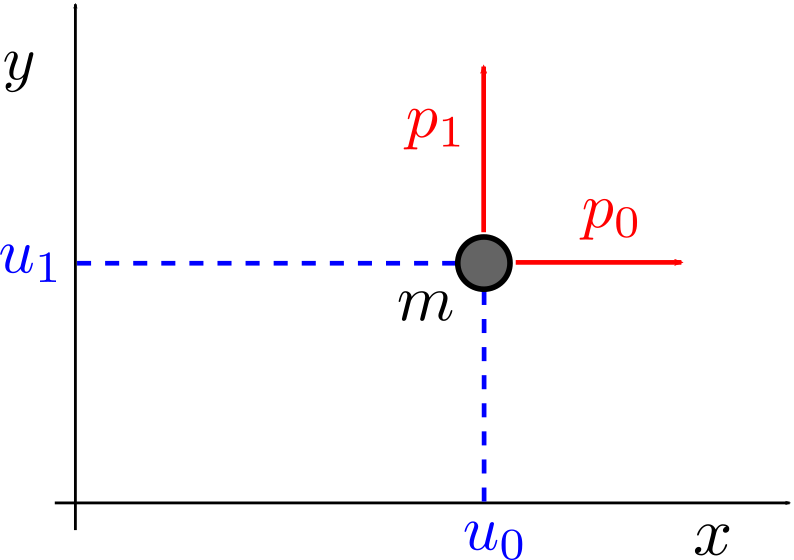
\includegraphics[width=0.4\textwidth]{figures/elements/mass-element}
\caption{Point mass element}
\label{fig:elements:point-mass}
\end{figure}

The equation of motion for this system can be written down directly by using Newton's second law of motion:

\begin{equation}
\underbrace{
\begin{bmatrix}
m & 0\\
0 & m
\end{bmatrix}
}_{\boldsymbol{M}}
\underbrace{
\begin{bmatrix}
\ddot{u}_0\\
\ddot{u}_1
\end{bmatrix}
}_{\boldsymbol{\ddot{u}}}
+
\underbrace{
\begin{bmatrix}
0\\
0
\end{bmatrix}
}_{\boldsymbol{q}(\boldsymbol{u},\,\dot{\boldsymbol{u}})}
=
\underbrace{
\begin{bmatrix}
p_0\\
p_1
\end{bmatrix}
}_{\boldsymbol{p}(t)}
\end{equation}

This immediately gives us the element's mass matrix, internal forces (which are zero) and external forces.
Because the internal forces are zero, the tangent stiffness and damping matrices are zero as well:

\begin{equation}
\boldsymbol{K} = \frac{\partial \boldsymbol{q}}{\partial \boldsymbol{u}} =
\begin{bmatrix}
0 & 0\\
0 & 0
\end{bmatrix},
\quad
\boldsymbol{D} = \frac{\partial \boldsymbol{q}}{\partial \dot{\boldsymbol{u}}} =
\begin{bmatrix}
0 & 0\\
0 & 0
\end{bmatrix}
\end{equation}

\newpage
\section{Beam Element (Co-Rotational)}

\textcolor{red}{TODO: Short outline of the co-rotational approach.}

\newpage
\subsection{Castigliano's Second Theorem}

This section provides a short recapitulation of Castigliano's second theorem, which we are going to use for deriving the linear part of our beam element.
Castigliano's second theorem can be used for computing the displacements of arbitrary linear-elastic structures.
It is stated as follows:

\textcolor{red}{TODO: Quote from Wikipedia}
If the strain energy of a linearly elastic structure can be expressed as a function of generalised force Qi then the partial derivative of the strain energy with respect to generalised force gives the generalised displacement qi in the direction of Qi.

To illustrate this theorem, let's consider a simple bar as shown in figure \ref{fig:castigliano-bar-1}.
It has an initial length of $l$ and a variable longitudinal stiffness $EA(s)$ with $s \in [0,\,l]$.
The first part of this exercise is to compute the displacement $u$ at the end of the bar where the force $F$ is applied.

\begin{figure}[h]
\centering
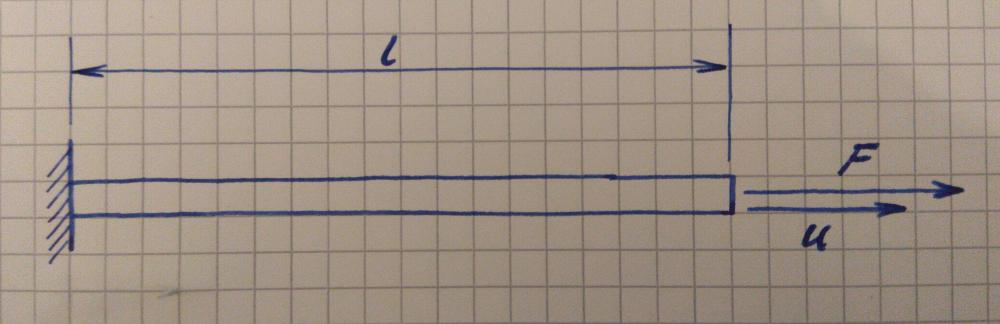
\includegraphics[width=0.5\textwidth]{figures/elements/castigliano-bar-1.jpg}
\caption{Bar of length $l$ with a load $F$ at the end}
\label{fig:castigliano-bar-1}
\end{figure}

First of all, the strain energy of a bar is given by

\begin{equation}
\Pi = \frac{1}{2}\int_{0}^{l}\frac{N^2}{EA}\,ds
\end{equation}

where $N(s)$ is the normal force of the cross sections along the length of the bar.
In this case it is easy to see that we have a constant normal force of $N(s) = F$.
According to Castigliano's theorem, the displacement $u$ in the direction of the force is

\begin{equation}
u = \frac{\partial \Pi}{\partial F} = \frac{\partial}{\partial F}\left(\frac{1}{2}\int_{0}^{l}\frac{F^2}{EA}\,ds\right) = \underbrace{\left(\int_{0}^{l}\frac{1}{EA}\,ds\right)}_{K^{-1}}F.
\end{equation}

By this we have identified the inverse $K^{-1}$ of the stiffness of the bar at that point and direction.
It is an integral over the length of the bar that takes the exact distribution of longitudinal stiffness into account.
If we assume $EA$ as constant for a quick sanity check, we get a stiffness of $K = \frac{EA}{l}$, which is the well known result for the stiffness of a bar.

It is especially worth mentioning that we arrived at this result without any kinematic considerations, i.e. we didn't have to think about the distribution of strain in the bar due to the normal force and how that relates to the displacement $u$, which makes the method very simple and elegant.
One apparent shortcoming of the method is that it only gives us the displacement at the end of the bar, where the external force is applied, and nowhere else.
This limitation can be worked around by introducing additional "imaginary" forces at other points of interest and setting them to zero after having calculated the associated displacements.

As part two of this exercise, let's calculate the displacement $\overline{u}$ at an arbitrary point $\overline{s}$ within the bar as shown in figure \ref{fig:castigliano-bar-2} by introducing the imaginary auxiliary force $\overline{F} = 0$.

\begin{figure}[h]
\centering
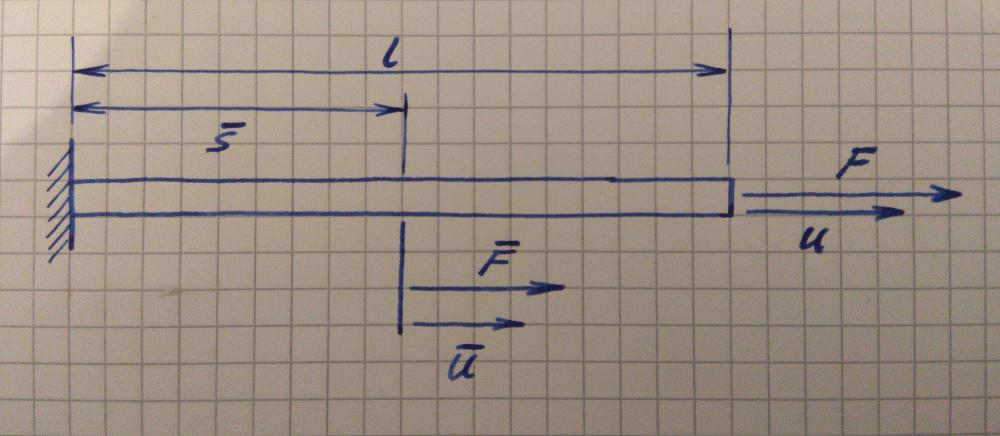
\includegraphics[width=0.5\textwidth]{figures/elements/castigliano-bar-2.jpg}
\caption{Bar of length $l$ with a load $F$ at the end and auxiliary force $\overline{F}$}
\label{fig:castigliano-bar-2}
\end{figure}

First of all, the distribution of normal force is now given by the piecewise function

\begin{equation}
N(s) = \begin{cases}
F + \overline{F}, & \text{if}\ \ 0 \le s < \overline{s} \\
F, & \text{if}\ \ \overline{s} \le s \le l \\
\end{cases}
\end{equation}

Therefore the potential elastic energy becomes
%
\begin{align}
\Pi &= \frac{1}{2}\int_{0}^{l}\frac{N^2}{EA}\,ds = \frac{1}{2}\left(\int_{0}^{\overline{s}}\frac{(F + \overline{F})^2}{EA}\,ds + \int_{\overline{s}}^{l}\frac{F^2}{EA}\,ds\right) \\
\end{align}

Application of Castigliano's theorem yields the displacement $\overline{u}$ depending on the forces $F$ and $\overline{F}$.
The actual displacement is obtained by setting the auxiliary force $\overline{F}$ to zero.
%
\begin{align}
\overline{u} &= \frac{\partial \Pi}{\partial \overline{F}} = \frac{\partial}{\partial \overline{F}}\left( \frac{1}{2} \int_{0}^{\overline{s}}\frac{(F + \overline{F})^2}{EA}\,ds \right) = \left(\int_{0}^{\overline{s}}\frac{1}{EA}\,ds \right)\left(F + \overline{F}\right) \\
&= \left(\int_{0}^{\overline{s}}\frac{1}{EA}\,ds \right)F.
\end{align}

This way we got the complete displacement distribution within the bar.
In the next section we are going to use Castigliano's theorem for calculating the stiffness matrix and displacements of a linear-elastic beam segment.

\newpage
\subsection{Stiffness Matrix of a Beam Segment (3)}

\begin{figure}[h]
\centering
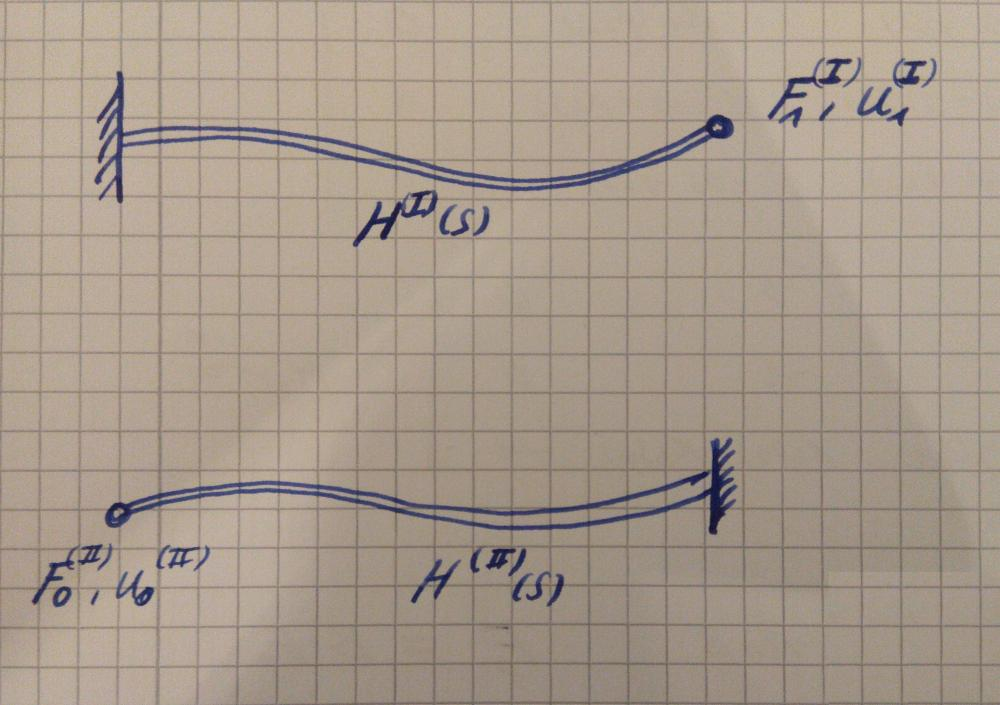
\includegraphics[width=0.5\textwidth]{figures/elements/castigliano-beam-cases.jpg}
\caption{Loading cases I and II}
\label{fig:castigliano-beam-cases}
\end{figure}

\subsubsection*{Loadcases}

The stiffness of the beam segment with respect to the combined nodal displacement and forces is

\begin{equation}
\underbrace{
\begin{bmatrix}
\boldsymbol{F}_0 \\
\boldsymbol{F}_1 \\
\end{bmatrix}
}_{\boldsymbol{F}}
=
\underbrace{
\begin{bmatrix}
\boldsymbol{K}_{0,0} & \boldsymbol{K}_{0,1} \\
\boldsymbol{K}_{1,0} & \boldsymbol{K}_{1,1} \\
\end{bmatrix}
}_{\boldsymbol{K}}
\underbrace{
\begin{bmatrix}
\boldsymbol{u}_0 \\
\boldsymbol{u}_1 \\
\end{bmatrix}
}_{\boldsymbol{u}}
\end{equation}

with the stiffness matrix $\boldsymbol{K} \in \mathbb{R}^{6 \times 6}$ and the four submatrices $\boldsymbol{K}_{ij} \in \mathbb{R}^{3 \times 3}$.
We can get a physical interpretation of the submatrices by constraining one of the nodes, ie. $\boldsymbol{u}_{0} = 0$ and $\boldsymbol{u}_{1} = 0$.

In the case $\boldsymbol{u}_{0} = 0$, which we will call case I, the resulting forces are

\begin{align}
\boldsymbol{F}_1 &= \boldsymbol{K}_{1,1}\,\boldsymbol{u}_1 \\
\boldsymbol{F}_0 &= \boldsymbol{K}_{0,1}\,\boldsymbol{u}_1
\end{align}

In the case $\boldsymbol{u}_{1} = 0$, which we will call case II, the resulting forces are

\begin{align}
\boldsymbol{F}_0 &= \boldsymbol{K}_{0,0}\,\boldsymbol{u}_0 \\
\boldsymbol{F}_1 &= \boldsymbol{K}_{1,0}\,\boldsymbol{u}_0
\end{align}

Put into words, the diagonal matrix blocks $\boldsymbol{K}_{0,0}$ and $\boldsymbol{K}_{1,1}$ relate the forces and displacements at a free node to each other, if the other node is restrained.
The off-diagonal blocks $\boldsymbol{K}_{1,0}$ and $\boldsymbol{K}_{0,1}$ relate the displacements at the free node to the forces at the restrained node.
This means that we can obtain the full stiffness matrix of the segment by analyzing those two distinct loadcases and assembling the partial results in the end.

The nodal forces $\boldsymbol{F}_0$ and $\boldsymbol{F}_1$ are not completely independent of each other, since they have to be in static equilibrium with each as a necessary condition for the element to be in equilibrium.
Balancing the forces and moments around node 1 gives us the three conditions
%
\begin{align}
x:\quad &F_{x,0} + F_{x,1} = 0 \\
y:\quad &F_{y,0} + F_{y,1} = 0 \\
z:\quad &M_{z,0} + M_{z,1} + F_{x,0}(y_1 - y_0) - F_{y,0}(x_1 - x_0) = 0
\end{align}

This can be written as the following matrix equation between the nodal forces,
%
\begin{align}
\boldsymbol{F}_0 &= \boldsymbol{B}_{0,1}\cdot\boldsymbol{F}_1 \\
\boldsymbol{F}_1 &= \boldsymbol{B}_{1,0}\cdot\boldsymbol{F}_0
\end{align}

with the matrix $\boldsymbol{B}_{i,j}$ defined as

\begin{equation}
\boldsymbol{B}_{i,j} = \begin{bmatrix}
-1 & 0 & 0 \\
0 & -1 & 0 \\
y_j - y_i & x_i - x_j & -1
\end{bmatrix}.
\end{equation}

We can use this relationship to calculate the forces at the clamped nodes in the cases I and II in order to obtain the off-diagonal stiffnesses $\boldsymbol{K}_{1,0}$ and $\boldsymbol{K}_{0,1}$ as follows,
%
\begin{align}
\boldsymbol{F}_0 &= \boldsymbol{B}_{0,1}\boldsymbol{F}_1 = \underbrace{\boldsymbol{B}_{0,1}\boldsymbol{K}_{1,1}}_{\boldsymbol{K}_{0,1}}\boldsymbol{u}_1 \\
\boldsymbol{F}_1 &= \boldsymbol{B}_{1,0}\boldsymbol{F}_0 = \underbrace{\boldsymbol{B}_{1,0}\boldsymbol{K}_{0,0}}_{\boldsymbol{K}_{1,0}}\boldsymbol{u}_0
\end{align}

In practive we only have to calculate one of the off-diagonal blocks since the complete stiffness matrix must be symmetric and therefore $\boldsymbol{K}_{1,0} = \boldsymbol{K}_{0,0}^\intercal$.
Since the off-diagonal stiffnesses have been shown to depend on the diagonal stiffnesses $\boldsymbol{K}_{0,0}$ and $\boldsymbol{K}_{1,1}$, the remaining task is to determine those matrices by analyzing the loadcases I and II, respectively.

\subsubsection*{Loadcase I}

The beam is clamped on the left and a force is applied at node 1.
Due to static equilibrium, the cross section forces in the beam for a force $\boldsymbol{F}_\eta$ that is applied at the length $s_\eta$ with $\eta \in [0,\,1]$ are

\begin{equation}
\underbrace{
\begin{bmatrix}
N \\ M \\ Q
\end{bmatrix}
}_{\boldsymbol{f}^{\mathrm{I}}_{\eta}(s)}
=
\underbrace{
\begin{bmatrix}
\cos(\varphi(s)) & \sin(\varphi(s)) & 0 \\
y(s) - y(s_\eta) & x(s_\eta) - x(s) & 1 \\
-\sin(\varphi(s)) & \cos(\varphi(s)) & 0 \\
\end{bmatrix}
}_{\boldsymbol{H}_{\eta}(s)}
\underbrace{
\begin{bmatrix}
F_{x,\eta} \\ F_{y,\eta} \\ M_{z,\eta}
\end{bmatrix}
}_{\boldsymbol{F}_\eta}. \label{eq:section-static-equilibrium}
\end{equation}

Combining the nodal force $\boldsymbol{F}_1$ at $s_1$ and the variable auxiliary force $\boldsymbol{F}_\eta$ at $s_\eta$:

\begin{equation}
\boldsymbol{f}^{\mathrm{I}}(s) = \begin{cases}
\boldsymbol{H}_{1}(s)\boldsymbol{F}_1 + \boldsymbol{H}_{\eta}(s)\boldsymbol{F}_\eta, & \text{if}\ \ s_0 \le s < s_\eta \\
\boldsymbol{H}_{1}(s)\boldsymbol{F}_1, & \text{if}\ \ s_\eta \le s \le s_1 \\
\end{cases}
\end{equation}

The potential energy for this loadcase is therefore

\begin{equation}
\Pi^{\mathrm{I}} = \frac{1}{2}\left(\int_{s_0}^{s_\eta} \left(\boldsymbol{H}_{1}\boldsymbol{F}_1 + \boldsymbol{H}_{\eta}\boldsymbol{F}_\eta\right)^\intercal\boldsymbol{C}^{-1}\left(\boldsymbol{H}_{1}\boldsymbol{F}_1 + \boldsymbol{H}_{\eta}\boldsymbol{F}_\eta\right)\,ds + \int_{s_\eta}^{s_1} \left(\boldsymbol{H}_{1}\boldsymbol{F}_1\right)^\intercal\boldsymbol{C}^{-1}\left(\boldsymbol{H}_{1}\boldsymbol{F}_1\right)\,ds\right)
\end{equation}

and the displacement $\boldsymbol{u}_\eta$ at position $s_\eta$

\begin{align}
\boldsymbol{u}^{\mathrm{I}}_\eta &= \frac{\partial \Pi^{\mathrm{I}}}{\partial \boldsymbol{F}_\eta}\Bigg|_{\boldsymbol{F}_\eta = 0} = \frac{\partial}{\partial \boldsymbol{F}_\eta}\left(\frac{1}{2}\int_{s_0}^{s_\eta} \left(\boldsymbol{H}_{1}\boldsymbol{F}_1 + \boldsymbol{H}_{\eta}\boldsymbol{F}_e\right)^\intercal\boldsymbol{C}^{-1}\left(\boldsymbol{H}_{1}\boldsymbol{F}_1 + \boldsymbol{H}_{\eta}\boldsymbol{F}_\eta\right)\,ds\right)\Bigg|_{\boldsymbol{F}_\eta = 0} \notag \\
&= \underbrace{\left(\int_{s_0}^{s_\eta} \boldsymbol{H}_\eta^\intercal\boldsymbol{C}^{-1}\boldsymbol{H}_1\,ds\right)}_{\boldsymbol{K}^{-1}_{1,\eta}}\boldsymbol{F}_1
\end{align}

The stiffness matrix $\boldsymbol{K}^{-1}_{1,1}$ for the right node follows for $\eta = 1$.

%Displacement at node 1 ($s_e = s_1$):
%
%\begin{align}
%\boldsymbol{u}^{(I)}_1 &= \underbrace{\left(\int_{s_0}^{s_e} \boldsymbol{H}_1^\intercal\boldsymbol{C}^{-1}\boldsymbol{H}_1\,ds\right)}_{\boldsymbol{K}^{-1}_{1,1}}\boldsymbol{F}_1
%\end{align}

\subsubsection*{Loadcase II}

\begin{equation}
\underbrace{
\begin{bmatrix}
N \\ M \\ Q
\end{bmatrix}
}_{\boldsymbol{f}^{\mathrm{II}}_{\eta}(s)}
=
\underbrace{
\begin{bmatrix}
-\cos(\varphi(s)) & -\sin(\varphi(s)) & 0 \\
y(s_\eta) - y(s) & x(s) - x(s_\eta) & -1 \\
\sin(\varphi(s)) & -\cos(\varphi(s)) & 0 \\
\end{bmatrix}
}_{-\boldsymbol{H}_{\eta}(s)}
\underbrace{
\begin{bmatrix}
F_{x,\eta} \\ F_{y,\eta} \\ M_{z,\eta}
\end{bmatrix}
}_{\boldsymbol{F}_\eta}. \label{eq:section-static-equilibrium}
\end{equation}

\begin{equation}
\boldsymbol{f}^{\mathrm{II}}(s) = \begin{cases}
-\boldsymbol{H}_{0}(s)\boldsymbol{F}_0, & \text{if}\ \ s_0 \le s \le s_\eta \\
-\boldsymbol{H}_{0}(s)\boldsymbol{F}_0 - \boldsymbol{H}_{\eta}(s)\boldsymbol{F}_\eta, & \text{if}\ \ s_\eta \le s < s_1 \\
\end{cases}
\end{equation}

\begin{equation}
\Pi^{\mathrm{II}} = \frac{1}{2}\left(\int_{s_0}^{s_\eta} \left(\boldsymbol{H}_{0}\boldsymbol{F}_0\right)^\intercal\boldsymbol{C}^{-1}\left(\boldsymbol{H}_{0}\boldsymbol{F}_0\right)\,ds + \int_{s_\eta}^{s_1} \left(\boldsymbol{H}_{0}\boldsymbol{F}_0 + \boldsymbol{H}_{\eta}\boldsymbol{F}_\eta\right)^\intercal\boldsymbol{C}^{-1}\left(\boldsymbol{H}_{0}\boldsymbol{F}_0 + \boldsymbol{H}_{\eta}\boldsymbol{F}_\eta\right)\,ds\right)
\end{equation}

\begin{align}
\boldsymbol{u}^{\mathrm{II}}_\eta &= \frac{\partial \Pi^{\mathrm{II}}}{\partial \boldsymbol{F}_\eta}\Bigg|_{\boldsymbol{F}_\eta = 0} = \frac{\partial}{\partial \boldsymbol{F}_\eta}\left(\frac{1}{2}\int_{s_\eta}^{s_1} \left(\boldsymbol{H}_{0}\boldsymbol{F}_0 + \boldsymbol{H}_{\eta}\boldsymbol{F}_\eta\right)^\intercal\boldsymbol{C}^{-1}\left(\boldsymbol{H}_{0}\boldsymbol{F}_0 + \boldsymbol{H}_{\eta}\boldsymbol{F}_\eta\right)\,ds\right)\Bigg|_{\boldsymbol{F}_\eta = 0} \notag \\
&= \underbrace{\left(\int_{s_\eta}^{s_1} \boldsymbol{H}_\eta^\intercal\boldsymbol{C}^{-1}\boldsymbol{H}_0\,ds\right)}_{\boldsymbol{K}^{-1}_{0,\eta}}\boldsymbol{F}_0
\end{align}

The stiffness matrix $\boldsymbol{K}^{-1}_{0,0}$ for the left node follows for $\eta = 0$.

%Displacement at node 1 ($s_e = s_1$):
%
%\begin{align}
%\boldsymbol{u}^{(II)}_0 &= \underbrace{\left(\int_{s_e}^{s_1} \boldsymbol{H}_0^\intercal\boldsymbol{C}^{-1}\boldsymbol{H}_0\,ds\right)}_{\boldsymbol{K}^{-1}_{0,0}}\boldsymbol{F}_0
%\end{align}

\subsubsection*{Combined Displacements}

Due to linear superposition \textcolor{red}{TODO: explain}, the displacements under forces at both nodes can be added as

\begin{equation}
\boldsymbol{u}_{\eta} = \boldsymbol{K}_{0,\eta}^{-1}\,\boldsymbol{F}_0 + \boldsymbol{K}_{1,\eta}^{-1}\,\boldsymbol{F}_1.
\end{equation}

Therefore the displacement evaluation matrix is

\begin{align}
\boldsymbol{u}_{\eta} &= \boldsymbol{K}_{0,\eta}^{-1}\boldsymbol{K}_{0,0}\boldsymbol{u}_0 + \boldsymbol{K}_{1,\eta}^{-1}\boldsymbol{K}_{1,1}\boldsymbol{u}_1 \\
&=
\underbrace{
\left[\boldsymbol{K}_{0,\eta}^{-1}\boldsymbol{K}_{0,0} \ \vert\ \boldsymbol{K}_{1,\eta}^{-1}\boldsymbol{K}_{1,1}\right]
}_{\boldsymbol{U}_\eta}
\begin{bmatrix}
\boldsymbol{u}_0 \notag \\
\boldsymbol{u}_1
\end{bmatrix} \notag \\
&=\boldsymbol{U}_\eta\boldsymbol{u}
\end{align}

We can simplify the computation of the matrices $\boldsymbol{K}_{0,\eta}^{-1}$ and $\boldsymbol{K}^{-1}_{1,\eta}$ by realizing that $\boldsymbol{H}_0$ and $\boldsymbol{H}_1$ are related by the static equilibrium matrix $\boldsymbol{B}_{i,j}$ \textcolor{red}{TODO: Link} as

\begin{equation}
\boldsymbol{H}_\eta(s) = -\boldsymbol{H}_0(s)\boldsymbol{B}_{\eta,0}
\end{equation}

This way, the flexibility matrices can be written as
%
\begin{align}
\boldsymbol{K}_{0,\eta}^{-1} &= -\boldsymbol{B}_{0,\eta}^\intercal\left(\int_{s_\eta}^{s_1} \boldsymbol{H}_0^\intercal\boldsymbol{C}^{-1}\boldsymbol{H}_0\,ds\right) \\
\boldsymbol{K}^{-1}_{1,\eta} &= \boldsymbol{B}_{0,\eta}^\intercal\left(\int_{s_0}^{s_\eta} \boldsymbol{H}_0^\intercal\boldsymbol{C}^{-1}\boldsymbol{H}_0\,ds\right)\boldsymbol{B}_{0,1}
\end{align}

so now there is only one function to be integrated, even though over different bounds, and the matrices for different $\eta$ are obtained by multiplying with the $\boldsymbol{B}$ matrices.
In the implementation, the integrand can be evaluated for each sub-interval between $s_0$ and $s_1$ and the partial results can be added as needed. \textcolor{red}{Better explanation?}

\subsubsection*{Combined Forces}

\begin{align}
\boldsymbol{f}(s) &= \boldsymbol{f}^{\mathrm{I}}(s) + \boldsymbol{f}^{\mathrm{II}}(s) \notag \\
&= \boldsymbol{H}_{1}(s)\boldsymbol{F}_1 - \boldsymbol{H}_{0}(s)\boldsymbol{F}_0 \notag \\
&= \begin{bmatrix}
-\boldsymbol{H}_{0}(s), & \boldsymbol{H}_{1}(s)
\end{bmatrix}
\boldsymbol{F} \notag \\
&= \begin{bmatrix}
-\boldsymbol{H}_{0}(s), & \boldsymbol{H}_{1}(s)
\end{bmatrix}
\boldsymbol{K}\boldsymbol{u} \notag \\
&= \begin{bmatrix}
\boldsymbol{H}_{1}\boldsymbol{K}_{1,0} - \boldsymbol{H}_{0}\boldsymbol{K}_{0,0}, & \boldsymbol{H}_{1}\boldsymbol{K}_{1,1} - \boldsymbol{H}_{0}\boldsymbol{K}_{0,1}
\end{bmatrix}\boldsymbol{u} \notag \\
\end{align}

%\newpage
%\subsection{Stiffness Matrix of a Beam Segment (2)}
%
%\subsubsection{Case I}
%
%Section forces when force $\boldsymbol{F}_e$ is applied at point $s_e$:
%
%\begin{equation}
%\underbrace{
%\begin{bmatrix}
%N \\ M \\ Q
%\end{bmatrix}
%}_{\boldsymbol{f}_e(s)}
%=
%\underbrace{
%\begin{bmatrix}
%\cos(\varphi(s)) & \sin(\varphi(s)) & 0 \\
%y(s) - y(s_e) & x(s_e) - x(s) & 1 \\
%-\sin(\varphi(s)) & \cos(\varphi(s)) & 0 \\
%\end{bmatrix}
%}_{\boldsymbol{H}_{e}(s)}
%\underbrace{
%\begin{bmatrix}
%F_{xe} \\ F_{ye} \\ M_{ze}
%\end{bmatrix}
%}_{\boldsymbol{F}_e}, \quad s \in [0,\,s_e]. \label{eq:section-static-equilibrium}
%\end{equation}
%
%Force $\boldsymbol{F}_1$ at $s_1$ and auxiliary force $\boldsymbol{F}_e$ at $s_e$:
%
%\begin{equation}
%\boldsymbol{f}^{(I)}(s) = \begin{cases}
%\boldsymbol{H}_{1}(s)\boldsymbol{F}_1 + \boldsymbol{H}_{e}(s)\boldsymbol{F}_e, & \text{if}\ \ s_0 \le s < s_e \\
%\boldsymbol{H}_{1}(s)\boldsymbol{F}_1, & \text{if}\ \ s_e \le s \le s_1 \\
%\end{cases}
%\end{equation}
%
%Elastic energy for case I:
%
%\begin{equation}
%\Pi^{(I)} = \frac{1}{2}\left(\int_{s_0}^{s_e} \left(\boldsymbol{H}_{1}\boldsymbol{F}_1 + \boldsymbol{H}_{e}\boldsymbol{F}_e\right)^\intercal\boldsymbol{C}^{-1}\left(\boldsymbol{H}_{1}\boldsymbol{F}_1 + \boldsymbol{H}_{e}\boldsymbol{F}_e\right)\,ds + \int_{s_e}^{s_1} \left(\boldsymbol{H}_{1}\boldsymbol{F}_1\right)^\intercal\boldsymbol{C}^{-1}\left(\boldsymbol{H}_{1}\boldsymbol{F}_1\right)\,ds\right)
%\end{equation}
%
%\begin{align}
%\boldsymbol{u}^{(I)}_e &= \frac{\partial \Pi^{(I)}}{\partial \boldsymbol{F}_e}\Bigg|_{\boldsymbol{F}_e = 0} = \frac{\partial}{\partial \boldsymbol{F}_e}\left(\frac{1}{2}\int_{s_0}^{s_e} \left(\boldsymbol{H}_{1}\boldsymbol{F}_1 + \boldsymbol{H}_{e}\boldsymbol{F}_e\right)^\intercal\boldsymbol{C}^{-1}\left(\boldsymbol{H}_{1}\boldsymbol{F}_1 + \boldsymbol{H}_{e}\boldsymbol{F}_e\right)\,ds\right)\Bigg|_{\boldsymbol{F}_e = 0} \notag \\
%&= \underbrace{\left(\int_{s_0}^{s_e} \boldsymbol{H}_e^\intercal\boldsymbol{C}^{-1}\boldsymbol{H}_1\,ds\right)}_{\boldsymbol{K}^{-1}_{1,e}}\boldsymbol{F}_1
%\end{align}
%
%Displacement at node 1 ($s_e = s_1$):
%
%\begin{align}
%\boldsymbol{u}^{(I)}_1 &= \underbrace{\left(\int_{s_0}^{s_e} \boldsymbol{H}_1^\intercal\boldsymbol{C}^{-1}\boldsymbol{H}_1\,ds\right)}_{\boldsymbol{K}^{-1}_{1,1}}\boldsymbol{F}_1
%\end{align}
%
%\newpage
%\subsubsection{Case II}
%
%Force $\boldsymbol{F}_0$ at $s_0$ and auxiliary force $\boldsymbol{F}_e$ at $s_e$: Can be derived from $\Pi^{(I)}$ by setting $\boldsymbol{F}_1 = \boldsymbol{B}\boldsymbol{F}_0$:
%
%\begin{equation}
%\boldsymbol{f}^{(II)}(s) = \begin{cases}
%\boldsymbol{H}_{1}(s)\boldsymbol{F}_1 + \boldsymbol{H}_{e}(s)\boldsymbol{F}_e, & \text{if}\ \ s_0 \le s < s_e \\
%\boldsymbol{H}_{1}(s)\boldsymbol{F}_1, & \text{if}\ \ s_e \le s \le s_1 \\
%\end{cases}
%\end{equation}
%
%
%
%\begin{equation}
%\Pi^{(II)} = \frac{1}{2}\left(\int_{s_0}^{s_e} \left(\boldsymbol{H}_{1}\boldsymbol{B}\boldsymbol{F}_0 + \boldsymbol{H}_{e}\boldsymbol{F}_e\right)^\intercal\boldsymbol{C}^{-1}\left(\boldsymbol{H}_{1}\boldsymbol{B}\boldsymbol{F}_0 + \boldsymbol{H}_{e}\boldsymbol{F}_e\right)\,ds + \int_{s_e}^{s_1} \left(\boldsymbol{H}_{1}\boldsymbol{B}\boldsymbol{F}_0\right)^\intercal\boldsymbol{C}^{-1}\left(\boldsymbol{H}_{1}\boldsymbol{B}\boldsymbol{F}_0\right)\,ds\right)
%\end{equation}
%
%(Wrong derivation, final result is a conjecture...)
%
%\begin{align}
%\boldsymbol{u}^{(II)}_e &= \frac{\partial \Pi^{(II)}}{\partial \boldsymbol{F}_e}\Bigg|_{\boldsymbol{F}_e = 0} = \frac{\partial}{\partial \boldsymbol{F}_e}\left(\frac{1}{2}\int_{s_0}^{s_e} \left(\boldsymbol{H}_{1}\boldsymbol{B}\boldsymbol{F}_0 + \boldsymbol{H}_{e}\boldsymbol{F}_e\right)^\intercal\boldsymbol{C}^{-1}\left(\boldsymbol{H}_{1}\boldsymbol{B}\boldsymbol{F}_0 + \boldsymbol{H}_{e}\boldsymbol{F}_e\right)\,ds\right)\Bigg|_{\boldsymbol{F}_e = 0} \notag \\
%&= \underbrace{\left(\int_{s_0}^{s_e} \boldsymbol{H}_e^\intercal\boldsymbol{C}^{-1}\boldsymbol{H}_1\,ds\right)\boldsymbol{B}}_{\boldsymbol{K}^{-1}_{1,e}}\boldsymbol{F}_1
%\end{align}
%
%Displacement at node 0 ($s_e = s_0$):
%
%\begin{align}
%\boldsymbol{u}^{(II)}_0 &= \underbrace{\left(\int_{s_0}^{s_e} \boldsymbol{H}_1^\intercal\boldsymbol{C}^{-1}\boldsymbol{H}_1\,ds\right)}_{\boldsymbol{K}^{-1}_{1,1}}\boldsymbol{F}_1
%\end{align}

\newpage
\subsection{Stiffness Matrix of a Beam Segment}

In this section we will derive the analytical stiffness matrix for a curved beam segment with arbitrary cross section properties that is also shear-deformable.
The only assumption we will make is that all displacements are small, so that we can apply linear-elastic theory to the problem.

\begin{figure}[h]
\centering
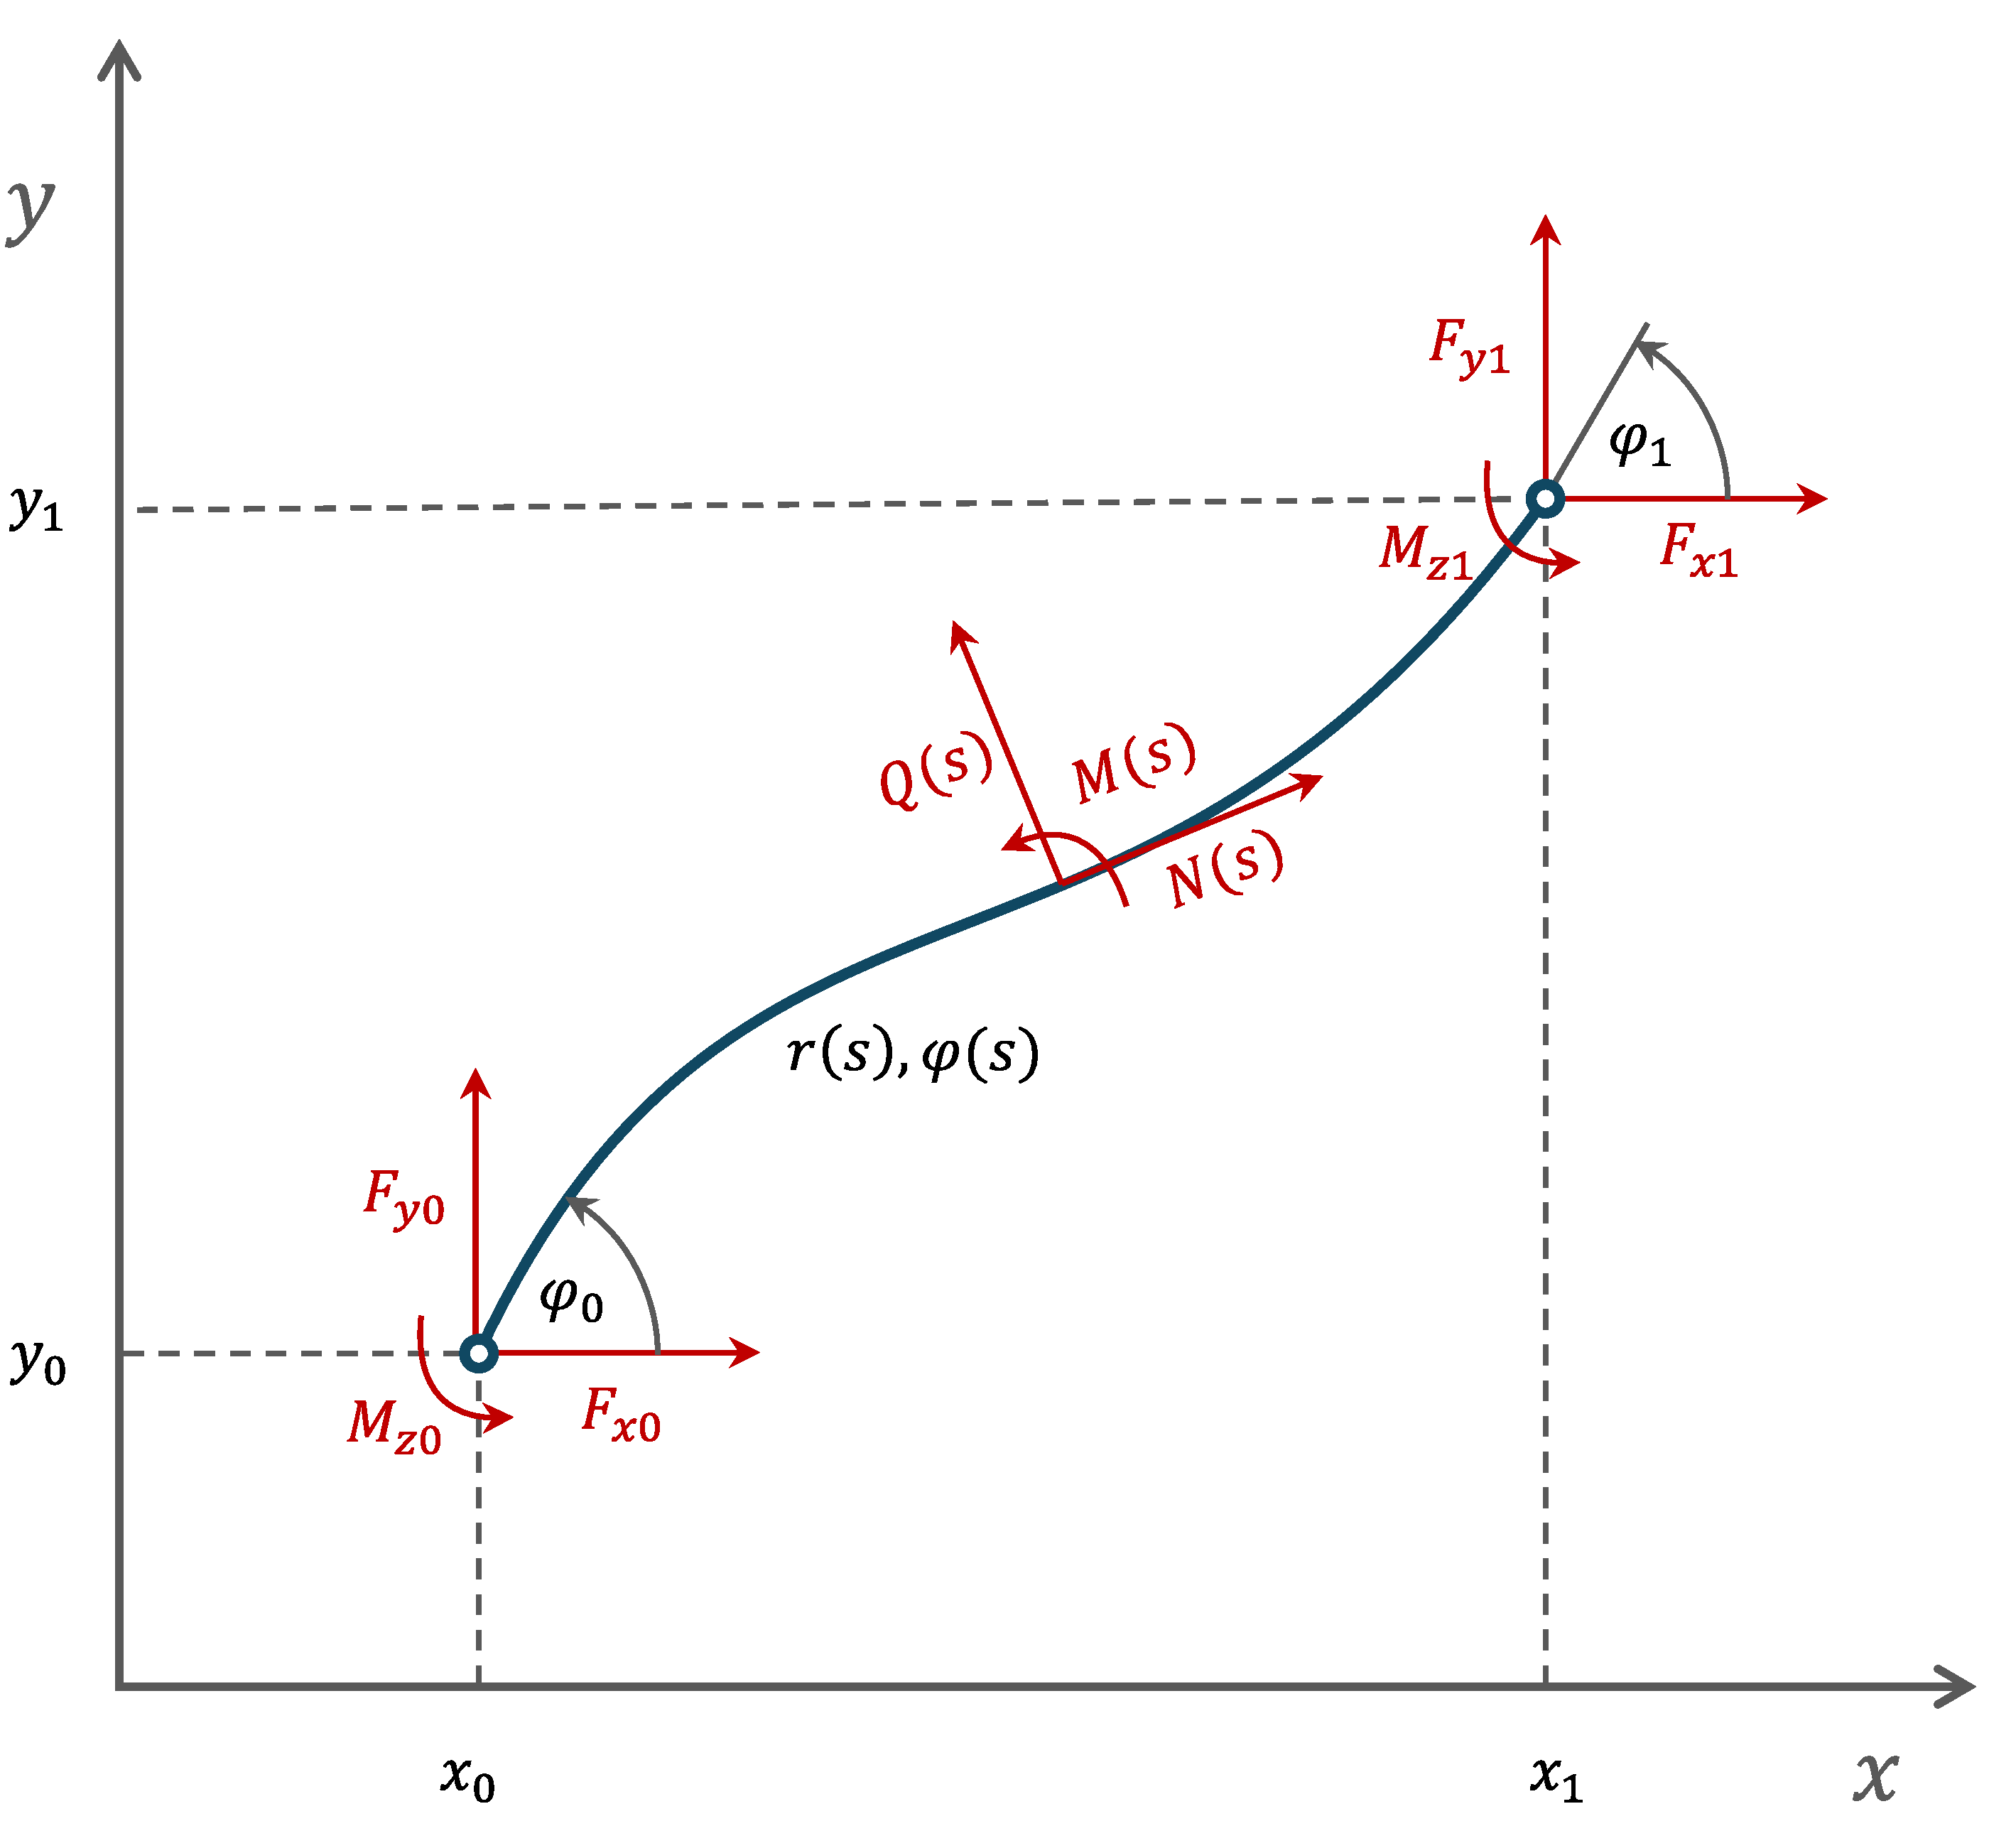
\includegraphics[width=0.5\textwidth]{figures/elements/beam-segment-linear}
\caption{Arbitrary beam segment with two nodes}
\label{fig:beam-segment-linear}
\end{figure}

Consider the beam segment shown in figure $\ref{fig:beam-segment-linear}$.
Its shape is described by the undeformed reference curve $\boldsymbol{r}(s) = \left[x(s),\,y(s)\right]^\intercal$ and the associated orientation angle $\varphi(s)$, where the parameter $s \in [s_0,\,s_1]$ is the arc length along the curve.

The stiffness properties of the cross sections are described by the cross sectional stiffness matrix $\boldsymbol{C}(s) \in \mathbb{R}^{3 \times 3}$ that is assumed to be known and establishes a linear constitutive relation of the form

\begin{equation}
\underbrace{
\begin{bmatrix}
N \\
M \\
Q \\
\end{bmatrix}
}_{\boldsymbol{f}(s)}
=
\underbrace{
\begin{bmatrix}
C_{\varepsilon\varepsilon} & C_{\varepsilon\kappa} & C_{\varepsilon\gamma} \\
C_{\varepsilon\kappa} & C_{\kappa\kappa} & C_{\kappa\gamma} \\
C_{\varepsilon\gamma} & C_{\kappa\gamma} & C_{\gamma\gamma} \\
\end{bmatrix}
}_{\boldsymbol{C}(s)}
\underbrace{
\begin{bmatrix}
\varepsilon \\
\kappa \\
\gamma \\
\end{bmatrix}
}_{\boldsymbol{e}(s)} \label{eq:section-stiffness-matrix}
\end{equation}

between the cross section forces~$\boldsymbol{f}$ and the generalized strains~$\boldsymbol{e}$.
The cross section forces consist of the normal force~$N$, the bending moment~$M$ and the shear force~$Q$ as shown in figure~\ref{fig:beam-segment-linear} while the strains consist of the elongation~$\varepsilon$ and the curvature~$\kappa$ of the beam axis as well as the shear angle~$\gamma$ between the section and the beam axis.

We assign two nodes to this segment, one on the starting point and one on the endpoint of the curve.
Each node is given two translational degrees of freedom in x- and y-direction and an angular degree of freedom around the z-axis.
At each node, the respective forces and moments

\begin{equation}
\boldsymbol{F}_{0} = \begin{bmatrix}
F_{x0} \\ F_{y0} \\ M_{z0}
\end{bmatrix},
\quad
\boldsymbol{F}_{1} = \begin{bmatrix}
F_{x1} \\ F_{y1} \\ M_{z1}
\end{bmatrix}
\end{equation}

are applied, to which the beam segment reacts with the (small) displacements

\begin{equation}
\boldsymbol{u}_{0} = \begin{bmatrix}
\Delta x_0 \\ \Delta y_0 \\ \Delta \varphi_0
\end{bmatrix},
\quad
\boldsymbol{u}_{1} = \begin{bmatrix}
\Delta x_1 \\ \Delta y_1 \\ \Delta \varphi_1
\end{bmatrix}
\end{equation}

in the respective directions of the forces/moments and relative to the initial state.
The goal is now to find the stiffness matrix of the segment, which describes the linear relationship between those forces and displacements.
We will do this by following the approach outlined in~\cite{bib:curved-beam-stiffness-matrix}, which is based on Castigliano's theorem, an energy-based method for calculating displacements of linear-elastic structures.

We start with a simple static consideration of the nodal forces.
In order for the segment to be in static equilibrium, the nodal forces have to fulfill the following conditions,
%
\begin{align}
x:\quad &F_{x0} + F_{x1} = 0 \\
y:\quad &F_{y0} + F_{y1} = 0 \\
z:\quad &M_{z0} + M_{z1} + F_{x0}\Delta y - F_{y0}\Delta x = 0
\end{align}

where~$\Delta x = x_1 - x_0$ and~$\Delta y = y_1 - y_0$.
This can be rearranged into a matrix equation that relates the forces on node 1 to those on node 0,

\begin{equation}
\underbrace{
\begin{bmatrix}
F_{x1} \\
F_{y1} \\
M_{z1} \\
\end{bmatrix}
}_{\boldsymbol{F}_1}
=
\underbrace{
\begin{bmatrix}
-1 & 0 & 0 \\
0 & -1 & 0 \\
-\Delta y & \Delta x & -1 \\
\end{bmatrix}
}_{\boldsymbol{B}}
\underbrace{
\begin{bmatrix}
F_{x0} \\
F_{y0} \\
M_{z0} \\
\end{bmatrix}
}_{\boldsymbol{F}_0}, \label{eq:segment-static-equilibrium}
\end{equation}

leaving only three independent nodal forces.
In a similar manner we can express the cross section forces $N(s)$, $M(s)$ and $Q(s)$ along the lenth of the segment in terms of the forces applied on node 1 by requiring the sections to be in static equilibrium with the applied forces.
This results in

\begin{equation}
\underbrace{
\begin{bmatrix}
N \\ M \\ Q
\end{bmatrix}
}_{\boldsymbol{f}(s)}
=
\underbrace{
\begin{bmatrix}
\cos(\varphi(s)) & \sin(\varphi(s)) & 0 \\
y(s) - y_1 & x_1 - x(s) & 1 \\
-\sin(\varphi(s)) & \cos(\varphi(s)) & 0 \\
\end{bmatrix}
}_{\boldsymbol{H}(s)}
\underbrace{
\begin{bmatrix}
F_{x1} \\ F_{y1} \\ M_{z1}
\end{bmatrix}
}_{\boldsymbol{F}_1}. \label{eq:section-static-equilibrium}
\end{equation}

Another prerequisite is the potential elastic energy (strain energy) of the beam segment.
It can be evaluated by integrating the product $\boldsymbol{f}^\intercal\boldsymbol{e}$ of section forces and strains over the beam's length and using the stiffness relation (\ref{eq:section-stiffness-matrix}) to eliminate the unknown strains:

\begin{equation}
\Pi = \frac{1}{2}\int_{s_0}^{s_1} \boldsymbol{f}^\intercal\boldsymbol{e}\,ds = \frac{1}{2}\int_{s_0}^{s_1} \boldsymbol{f}^\intercal\boldsymbol{C}^{-1}\boldsymbol{f}\,ds.
\end{equation}

According to Castigliano's second theorem, the partial derivative of the strain energy of a linear-elastic structure with respect to an applied force/moment is equal to the displacement/rotation of the structure at that point.

Let's first consider a load case where node 0 is fixed and forces are applied at node 1 only.
In this case, using equation (\ref{eq:section-static-equilibrium}), the strain energy becomes

\begin{equation}
\Pi_1 = \frac{1}{2}\int_{s_0}^{s_1} \boldsymbol{f}^\intercal\boldsymbol{C}^{-1}\boldsymbol{f}\,ds = \frac{1}{2}\boldsymbol{F}_1^\intercal\left(\int_{s_0}^{s_1} \boldsymbol{H}^\intercal\boldsymbol{C}^{-1}\boldsymbol{H}\,ds\right)\boldsymbol{F}_1
\end{equation}

and therefore, according to Castigliano's theorem, the corresponding displacements are

\begin{equation}
\boldsymbol{u}_{1} = \frac{\partial \Pi_1}{\partial \boldsymbol{F}_1} = \underbrace{\left(\int_{s_0}^{s_1} \boldsymbol{H}^\intercal\boldsymbol{C}^{-1}\boldsymbol{H}\,ds\right)}_{\boldsymbol{K}_{11}^{-1}}\boldsymbol{F}_1 = \boldsymbol{K}_{11}^{-1}\boldsymbol{F}_1.
\end{equation}

With this we have identified the inverse stiffness matrix $\boldsymbol{K}_{11}^{-1}$ that relates forces and displacements on node 1 to each other in this restricted load case.
Let's now consider the opposite case, where node 1 is fixed and the forces are applied at node 0 only.

Using (\ref{eq:section-static-equilibrium}) and (\ref{eq:segment-static-equilibrium}) we can express the strain energy in terms of $\boldsymbol{F}_0$ as

\begin{equation}
\Pi_0 = \frac{1}{2}\int_{s_0}^{s_1} \boldsymbol{f}^\intercal\boldsymbol{C}^{-1}\boldsymbol{f}\,ds = \frac{1}{2}\boldsymbol{F}_0^\intercal\underbrace{\boldsymbol{B}^\intercal\left(\int_{s_0}^{s_1} \boldsymbol{H}^\intercal\boldsymbol{C}^{-1}\boldsymbol{H}\,ds\right)\boldsymbol{B}}_{\boldsymbol{B}^\intercal\boldsymbol{K_{11}^{-1}\boldsymbol{B}}}\boldsymbol{F}_0.
\end{equation}

With the same reasoning as before this gives us the displacements

\begin{equation}
\boldsymbol{u}_{0} = \frac{\partial \Pi_0}{\partial \boldsymbol{F}_0} = \underbrace{\boldsymbol{B}^\intercal\boldsymbol{K_{11}^{-1}\boldsymbol{B}}}_{\boldsymbol{K}_{00}^{-1}}\boldsymbol{F}_0 = \boldsymbol{K}_{00}^{-1}\boldsymbol{F}_0
\end{equation}

and the inverse stiffness matrix $\boldsymbol{\boldsymbol{K}_{00}^{-1}}$ for node 0 in the considered configuration.
Since we are dealing with linear elasticity, we can use linear superposition of both of those load cases in order to get the overall stiffness relation of the beam segment.
We are however still missing the coupling between the nodes, i.e. the relationship between forces on node 0 and displacements on node 1 and vice versa.
For this we can use the static relationship~(\ref{eq:segment-static-equilibrium}) and the definition of the stiffness matrix to get
%
\begin{align}
\boldsymbol{F}_1 &= \boldsymbol{B}\boldsymbol{F}_0 = \underbrace{\boldsymbol{B}\boldsymbol{K}_{00}}_{\boldsymbol{K}_{10}}\boldsymbol{u}_0 = \boldsymbol{K}_{10}\boldsymbol{u}_0.
\end{align}

Due to symmetry we know that the second coupling stiffness must be $\boldsymbol{K}_{01} = \boldsymbol{K}_{10}^\intercal$.
Finally we add the forces from both load cases, which results in the complete stiffness relation for the beam segment as

\begin{equation}
\underbrace{
\begin{bmatrix}
\boldsymbol{F}_0 \\ \boldsymbol{F}_1
\end{bmatrix}
}_{\boldsymbol{F}}
=
\underbrace{
\begin{bmatrix}
\boldsymbol{K}_{00} & \boldsymbol{K}_{10}^\intercal \\
\boldsymbol{K}_{10} & \boldsymbol{K}_{11}
\end{bmatrix}
}_{\boldsymbol{K}}
\underbrace{
\begin{bmatrix}
\boldsymbol{u}_0 \\ \boldsymbol{u}_1
\end{bmatrix}
}_{\boldsymbol{u}} \label{eq:segment-stiffness-matrix}
\end{equation}

with the complete $6 \times 6$ stiffness matrix $\boldsymbol{K}$.
Note that this is an exact result since no simplifications have been made within the linear-elastic beam theory.
The integral over the beam length that occurs in the calculation of the partial stiffness matrices accounts for any arbitrary shape and distribution of cross section properties within the segment.

In practive, however, those integrals are approximated numerically since the shape and cross section of the beam segments can become quite complicated.
But since the stiffness matrix is constant, its computation has to be done only once prior to the actual simulation and is therefore not very time-critical.
This in turn allows for using more accurate numerical integration methods with error control and small tolerances as opposed to the usual Gaussian quadrature rules often used in nonlinear finite element analysis.

\subsubsection*{Evaluation of section forces and strains}

The stiffness matrix relates the nodal forces and displacements to each other, but it doesn't tell us anything about what happens within the beam segment in terms of forces and strains.
For the section forces we can use equation (\ref{eq:section-static-equilibrium}) and the total stiffness equation (\ref{eq:segment-stiffness-matrix}) to get

\begin{equation}
\boldsymbol{f}(s) = \boldsymbol{H}(s)\boldsymbol{F}_{1} = \underbrace{\boldsymbol{H}(s)\left[\boldsymbol{K}_{10},\,\boldsymbol{K}_{11}\right]}_{\boldsymbol{E}_f(s)}\boldsymbol{u}.
\end{equation}

So the section forces at any length $s$ are linearly related to the nodal displacements~$\boldsymbol{u}$ via the matrix~$\boldsymbol{E}_f(s)$, which we will call the force evaluation matrix.
Knowing the cross section forces, the strains can be computed from (\ref{eq:section-stiffness-matrix}) by inverting the section's stiffness matrix,

\begin{equation}
\boldsymbol{e}(s) = \boldsymbol{C}^{-1}(s)\boldsymbol{f}(s) = \underbrace{\boldsymbol{C}^{-1}(s)\boldsymbol{E}_f(s)}_{\boldsymbol{E}_e(s)}\boldsymbol{u}.
\end{equation}

In this case the relation to the displacements~$\boldsymbol{u}$ is given by the strain evaluation matrix~$\boldsymbol{E}_e(s)$.
Both of these matrices can be pre-computed for certain points of interest within the beam segment.
The actual evaluation of forces and strains is then only a matrix multiplication with the current nodal displacements.

\newpage
\subsection*{Alternative Method for verification}

\textcolor{red}{TODO: Move to verification chapter and link properly}

As an alternative to the analytical solution by integration, the stiffness matrix of an arbitrarily shaped beam segment can be computed by approximating it with a number of straight beam elements of constant cross section.
First of all, divide the beam segment into $n$ elements with index $i = 0 \ldots n-1$.
The length $l_i$ and orientation angle $\alpha_i$ of each element is then given by

\begin{align}
l_{i} &= \left| r_{i+1} - r_{i} \right|, \\
\alpha_i &= \mathrm{arctan2}\left(\frac{y_{i+1} - y_{i}}{x_{i+1} - x_{i}}\right).
\end{align}

The stiffness matrix of a straight timoshenko beam element with a constant section stiffness $\boldsymbol{C} = \mathrm{diag}(EA,\,EI,\,GA_s)$ with longitudinal stiffness $EA$, bending stiffness $EI$ and shear stiffness $GA_s$ is well known \textcolor{red}{Reference?} in structural mechanics and reads

\begin{equation}
\renewcommand\arraystretch{1.5}
\overline{\boldsymbol{K}}_i = \begin{bmatrix}
 \frac{EA_i}{l_i} &                           0 &                                0 & -\frac{EA_i}{l_i} &                           0 &                                0 \\
            0 &  \frac{12EI_i}{l_i^3(1 + \Phi)} &        \frac{6EI_i}{l_i^2(1 + \Phi)} &             0 & -\frac{12EI_i}{l_i^3(1 + \Phi)} &        \frac{6EI_i}{l_i^2(1 + \Phi)} \\
            0 &   \frac{6EI_i}{l_i^2(1 + \Phi)} & \frac{EI_i(4 + \Phi)}{l_i(1 + \Phi)} &             0 &  -\frac{6EI_i}{l_i^2(1 + \Phi)} & \frac{EI_i(2 - \Phi)}{l_i(1 + \Phi)} \\
-\frac{EA_i}{l_i} &                           0 &                                0 &  \frac{EA_i}{l_i} &                           0 &                                0 \\
            0 & -\frac{12EI_i}{l_i^3(1 + \Phi)} &       -\frac{6EI_i}{l_i^2(1 + \Phi)} &             0 &  \frac{12EI_i}{l_i^3(1 + \Phi)} &       -\frac{6EI_i}{l_i^2(1 + \Phi)} \\
            0 &   \frac{6EI_i}{l_i^2(1 + \Phi)} & \frac{EI_i(2 - \Phi)}{l_i(1 + \Phi)} &             0 &  -\frac{6EI_i}{l_i^2(1 + \Phi)} & \frac{EI_i(4 + \Phi)}{l_i(1 + \Phi)} \\
\end{bmatrix}
\end{equation}

with the shear-related factor $\Phi = \frac{12EI}{GA_s l^2}$.
This stiffness matrix needs to be transformed by the transformation matrix

\begin{equation}
\renewcommand\arraystretch{1.5}
\boldsymbol{T}_i = \begin{bmatrix}
\phantom{-}\cos(\alpha_i) & \sin(\alpha_i) & 0 & 0 & 0 & 0 \\
          -\sin(\alpha_i) & \cos(\alpha_i) & 0 & 0 & 0 & 0 \\
                      0 &            0 & 1 & 0 & 0 & 0 \\
0 & 0 & 0 & \phantom{-}\cos(\alpha_i) & \sin(\alpha_i) & 0 \\
0 & 0 & 0 &           -\sin(\alpha_i) & \cos(\alpha_i) & 0 \\
0 & 0 & 0 &                       0 &            0 & 1 \\
\end{bmatrix}
\end{equation}

in order to account for the orientation angle $\alpha$ of each element.
This leads to the element stiffness matrices

\begin{equation}
\renewcommand\arraystretch{1.5}
\boldsymbol{K}_{i} = \boldsymbol{T}_i^\intercal\,\overline{\boldsymbol{K}}_i\,\boldsymbol{T} =
\begin{bmatrix}
\boldsymbol{K}_{00}^{(i)} & \boldsymbol{K}_{01}^{(i)} \\
\boldsymbol{K}_{10}^{(i)} & \boldsymbol{K}_{11}^{(i)} \\
\end{bmatrix}
\end{equation}

which we partitioned into four equal blocks.
Due to the interconnection of the elements, where the end node of one element is the starting node of the next one, the full stiffness matrix of the assembly is given by the following matrix of overlapping blocks,

\begin{equation}
\renewcommand\arraystretch{1.5}
\boldsymbol{K}_{\mathrm{full}} = \begin{bmatrix}
\ddots & \ddots \\
& \boldsymbol{K}_{11}^{(i-1)} + \boldsymbol{K}_{00}^{(i)} & \boldsymbol{K}_{01}^{(i)} & \\
& \boldsymbol{K}_{10}^{(i)} & \boldsymbol{K}_{11}^{(i)} + \boldsymbol{K}_{00}^{(i+1)} & \boldsymbol{K}_{01}^{(i+1)} \\
&                           & \boldsymbol{K}_{10}^{(i+1)} & \boldsymbol{K}_{11}^{(i+1)} + \boldsymbol{K}_{00}^{(i+2)} \\
&                           &                             &                                          \ddots & \ddots \\
\end{bmatrix}.
\end{equation}

This matrix has the dimension $3(n+1) \times 3(n+1)$ and relates the forces and displacements of all nodes to each other.
We are however only interested in the $6 \times 6$ stiffness matrix with respect to the first and last node of the assembly.
This can be achieved by something called a \textit{static reduction} or \textit{Guyan reduction}.

First of all, the full stiffness relation is partitioned as follows,

\begin{equation}
\begin{bmatrix}
\boldsymbol{F}_{1} \\
\boldsymbol{0} \\
\boldsymbol{F}_{3} \\
\end{bmatrix}
=
\underbrace{
\begin{bmatrix}
          \boldsymbol{K}_{11} &           \boldsymbol{K}_{12} & \boldsymbol{K}_{13} \\
\boldsymbol{K}_{12}^\intercal &           \boldsymbol{K}_{22} & \boldsymbol{K}_{23} \\
\boldsymbol{K}_{13}^\intercal & \boldsymbol{K}_{23}^\intercal & \boldsymbol{K}_{33} \\
\end{bmatrix}
}_{\boldsymbol{K}_{\mathrm{full}}}
\begin{bmatrix}
\boldsymbol{u}_{1} \\
\boldsymbol{u}_{2} \\
\boldsymbol{u}_{3} \\
\end{bmatrix}
\end{equation}

where $\boldsymbol{u}_1 \in \mathbb{R}^3$ are the displacements of the first node, $\boldsymbol{u}_3 \in \mathbb{R}^3$ are the displacements of the last node and $\boldsymbol{u}_2 \in \mathbb{R}^{3n-1}$ are the displacements of all the intermediate nodes.
Only the first and last nodes have a corresponding applied force $\boldsymbol{F}_{1}$ and $\boldsymbol{F}_{3}$ while the intermediate nodes are free of external forces.

From the second block equation we can calculate the equilibrium displacements $\boldsymbol{u}_{2}$ of the intermediate nodes in terms of the other displacements,
%
\begin{align}
0 &= \boldsymbol{K}_{12}^\intercal \boldsymbol{u}_1 + \boldsymbol{K}_{22}\boldsymbol{u}_2 + \boldsymbol{K}_{23}\boldsymbol{u}_3 \notag \\
\Rightarrow \boldsymbol{u}_2 &= -\boldsymbol{K}_{22}^{-1}(\boldsymbol{K}_{12}^\intercal \boldsymbol{u}_1 + \boldsymbol{K}_{23}\boldsymbol{u}_3).
\end{align}

Using this, the intermediate displacements can be eliminated from the first and third block equations,
%
\begin{align}
\boldsymbol{F}_1 &= \boldsymbol{K}_{11}\boldsymbol{u}_1 + \boldsymbol{K}_{11}\boldsymbol{u}_2 + \boldsymbol{K}_{11}\boldsymbol{u}_3 \notag \\
   &= \boldsymbol{K}_{11}\boldsymbol{u}_1 - \boldsymbol{K}_{11}\boldsymbol{K}_{22}^{-1}(\boldsymbol{K}_{11}^\intercal \boldsymbol{u}_1 + \boldsymbol{K}_{11}\boldsymbol{u}_3) + \boldsymbol{K}_{11}\boldsymbol{u}_3 \notag \\
   &= (\boldsymbol{K}_{11} - \boldsymbol{K}_{11}\boldsymbol{K}_{22}^{-1}\boldsymbol{K}_{11}^\intercal )\boldsymbol{u}_1 + (\boldsymbol{K}_{11} - \boldsymbol{K}_{11}\boldsymbol{K}_{22}^{-1}\boldsymbol{K}_{11})\boldsymbol{u}_3, \\
\notag \\
\boldsymbol{F}_3 &= \boldsymbol{K}_{11}^\intercal \boldsymbol{u}_1 + \boldsymbol{K}_{11}^\intercal \boldsymbol{u}_2 + \boldsymbol{K}_{33}\boldsymbol{u}_3 \notag \\
   &= \boldsymbol{K}_{11}^\intercal \boldsymbol{u}_1 - \boldsymbol{K}_{11}^\intercal \boldsymbol{K}_{22}^{-1}(\boldsymbol{K}_{11}^\intercal \boldsymbol{u}_1 + \boldsymbol{K}_{11}\boldsymbol{u}_3) + \boldsymbol{K}_{33}\boldsymbol{u}_3 \notag \\
   &= (\boldsymbol{K}_{11}^\intercal  - \boldsymbol{K}_{11}^\intercal \boldsymbol{K}_{22}^{-1}\boldsymbol{K}_{11}^\intercal )\boldsymbol{u}_1 + (\boldsymbol{K}_{33} - \boldsymbol{K}_{11}^\intercal \boldsymbol{K}_{22}^{-1}\boldsymbol{K}_{11})\boldsymbol{u}_3.
\end{align}

Finally, rearranging the forces $\boldsymbol{F}_1$ and $\boldsymbol{F}_3$ and the corresponding displacements back into the matrix form

\begin{equation}
\renewcommand\arraystretch{1.5}
\begin{bmatrix}
\boldsymbol{F}_{1} \\
\boldsymbol{F}_{3} \\
\end{bmatrix}
=
\underbrace{
\begin{bmatrix}
\boldsymbol{K}_{11} - \boldsymbol{K}_{12}\boldsymbol{K}_{22}^{-1}\boldsymbol{K}_{12}^\intercal   &   \boldsymbol{K}_{13} - \boldsymbol{K}_{12}\boldsymbol{K}_{22}^{-1}\boldsymbol{K}_{23} \\
\boldsymbol{K}_{13}^\intercal - \boldsymbol{K}_{23}^\intercal \boldsymbol{K}_{22}^{-1}\boldsymbol{K}_{12}^\intercal & \boldsymbol{K}_{33} - \boldsymbol{K}_{23}^\intercal \boldsymbol{K}_{22}^{-1}\boldsymbol{K}_{23}
\end{bmatrix}
}_{\boldsymbol{K}_{\mathrm{red}}}
\begin{bmatrix}
\boldsymbol{u}_{1} \\
\boldsymbol{u}_{3} \\
\end{bmatrix}
\end{equation}

reveals the reduced stiffness matrix $\boldsymbol{K}_{\mathrm{red}} \in \mathbb{R}^{6 \times 6}$ as the final result.
Some quick benchmarks have shown that this method is less efficient than the numerical integration if high precision is required (i.e. large numbers of elements).
That's why it is used for verification only.

\newpage
\subsection{Local Frame of Reference}

As a first step towards a corotational formulation, a local frame of reference that moves along with the element is introduced as shown in figure \ref{fig:beam-element-frame}.
The origin of this frame is placed at the first node $(x_0,\,y_0)$ with the x-axis passing through the second node.

\begin{figure}[h]
\centering
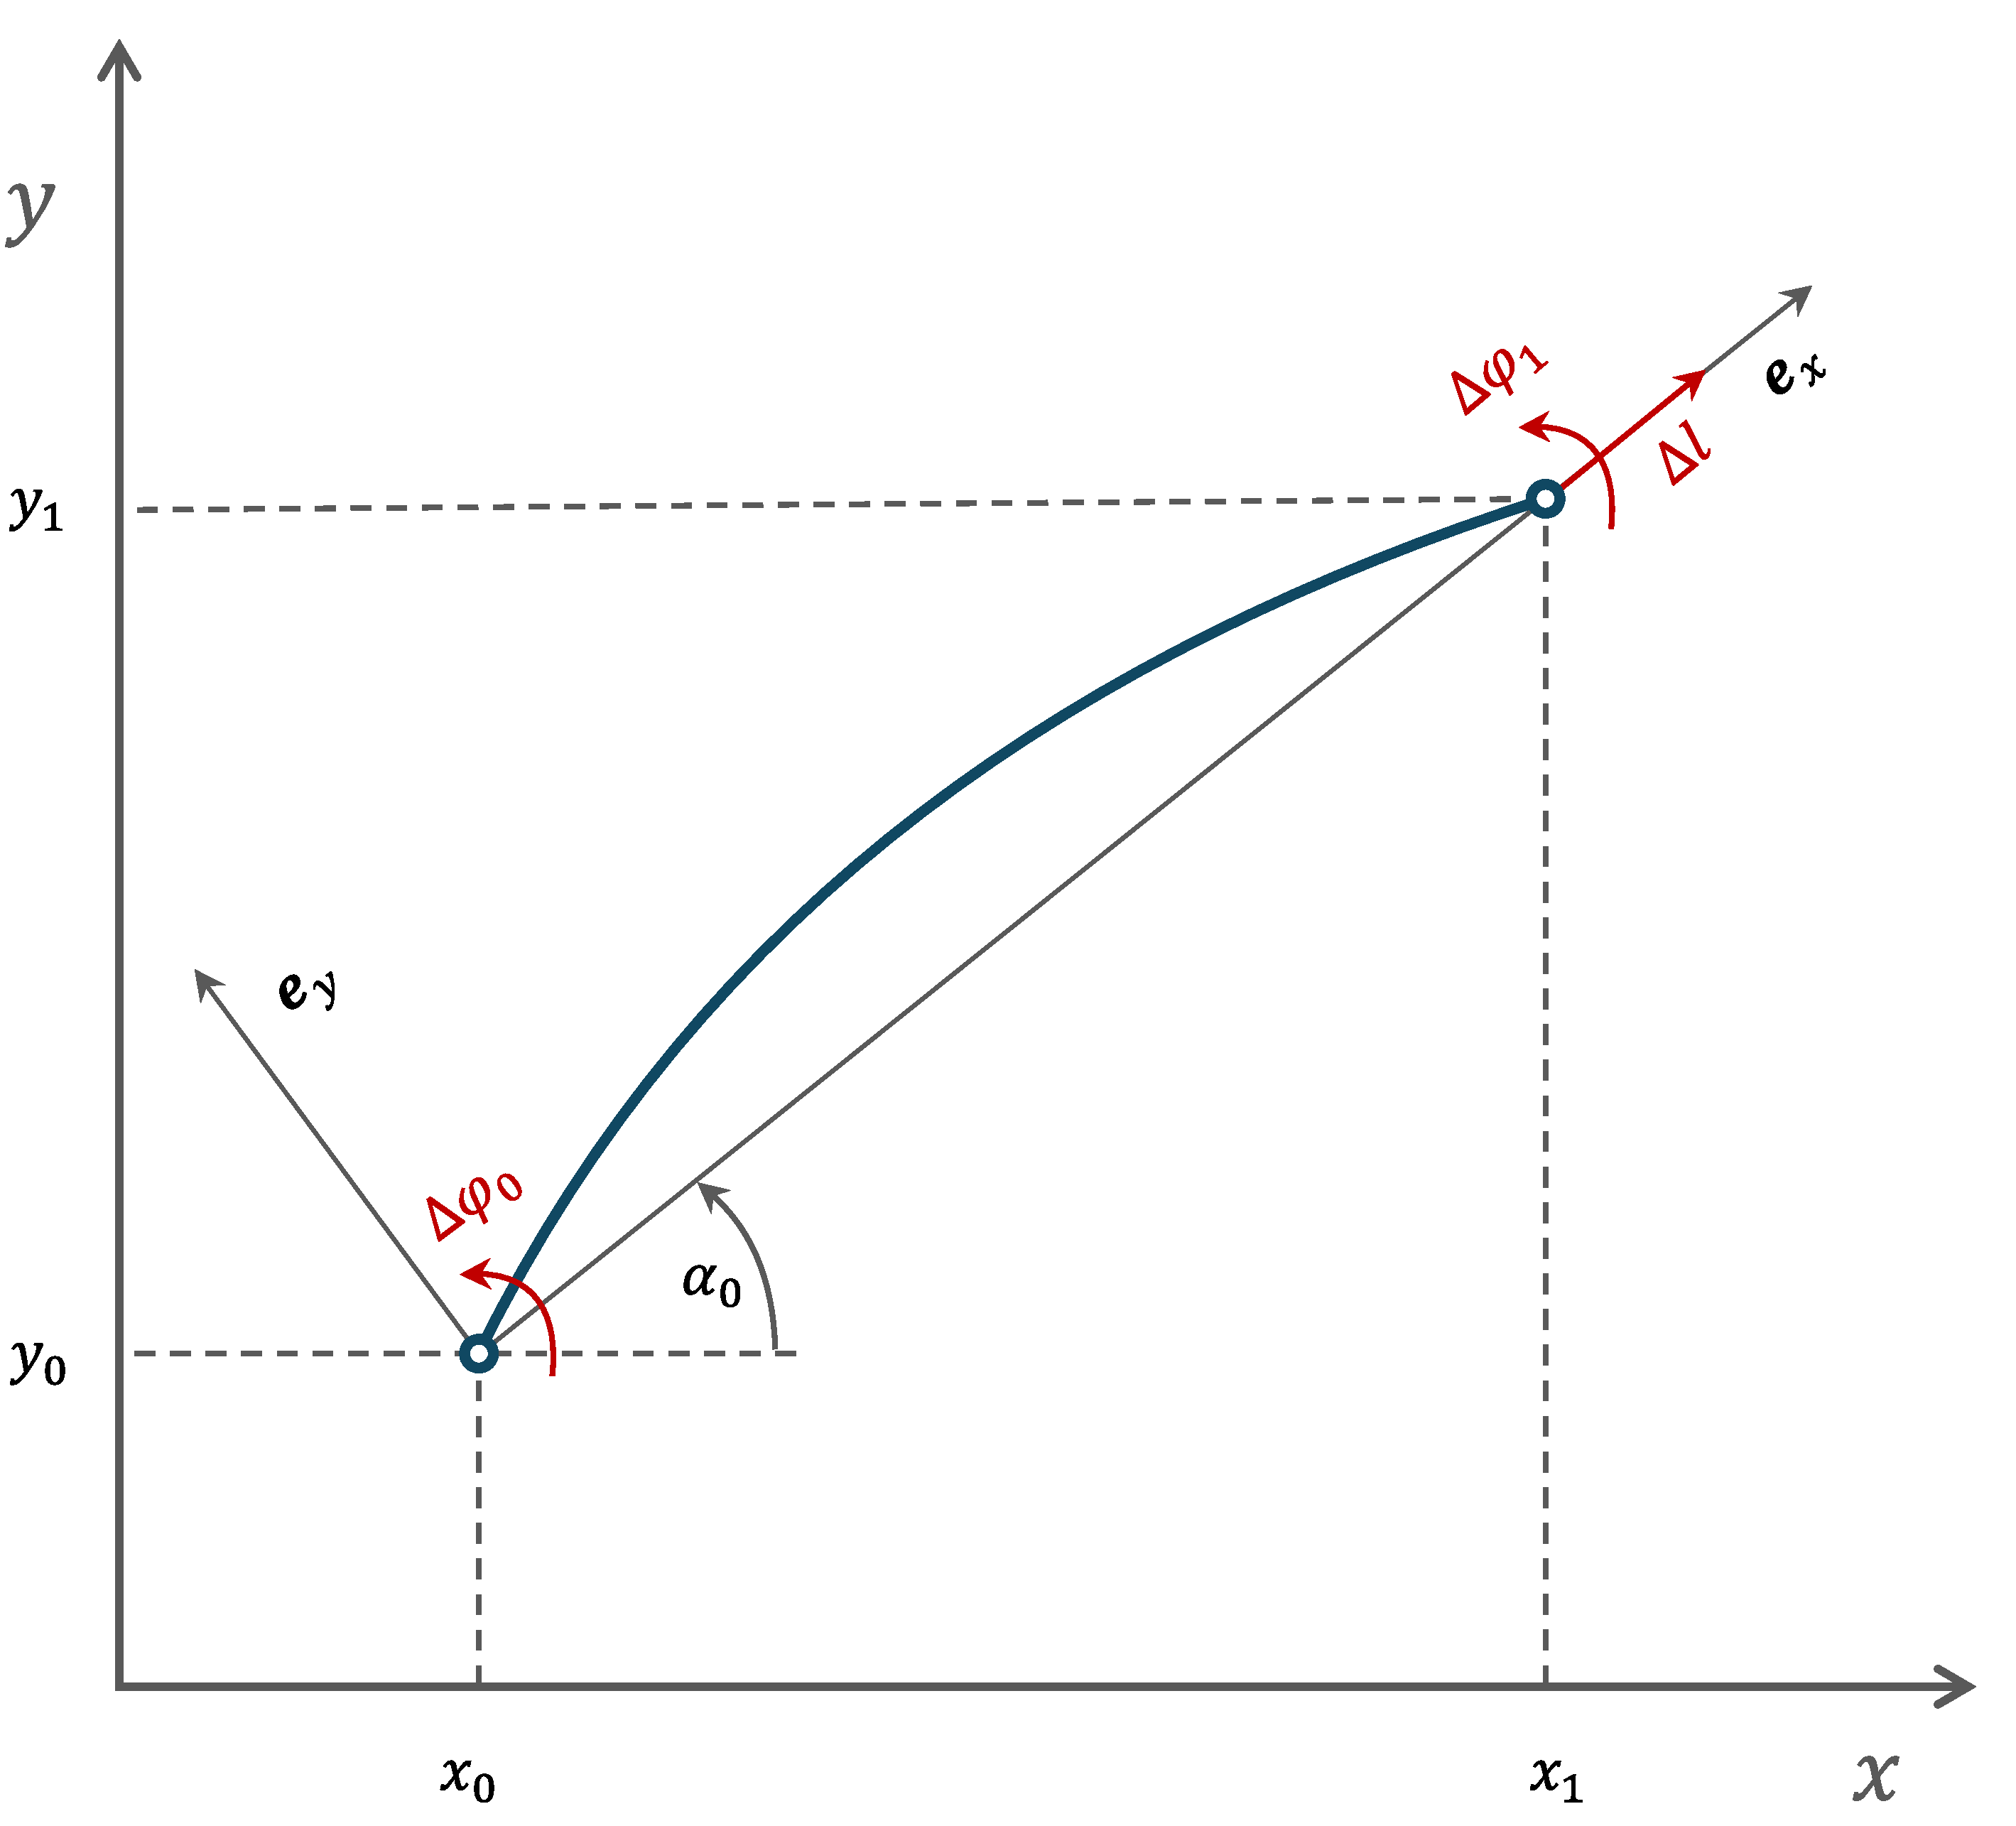
\includegraphics[width=0.5\textwidth]{figures/elements/beam-element-frame.pdf}
\caption{Local reference frame}
\label{fig:beam-element-frame}
\end{figure}

The x-axis can therefore be defined by the normalized direction vector

\begin{equation}
\boldsymbol{t} = \frac{\boldsymbol{r}_1 - \boldsymbol{r}_0}{\left|\boldsymbol{r}_1 - \boldsymbol{r}_0\right|}.
\end{equation}

To describe the elastic deformation of the element relative to this reference frame, three displacement coordinates are needed.
This is because the beam segment's position and rotation is now fixed with respect to the moving reference frame, taking away three of the original six degrees of freedom.
We choose the elastic displacements

\begin{equation}
\boldsymbol{u}_{e} = \begin{bmatrix}
\Delta l \\
\Delta \varphi_0 \\
\Delta \varphi_1 \\
\end{bmatrix}
\end{equation}

where $\Delta l$ is the elongation of the element along the local x-axis and $\Delta \varphi_0$, $\Delta \varphi_1$ are the changes in rotation angle at the two nodes.
The original displacements $\Delta\boldsymbol{u}$ of the beam segment can be expressed in terms of the new displacements as

\begin{equation}
\boldsymbol{u} =
\begin{bmatrix}
\Delta x_0 \\ \Delta y_0 \\ \Delta \varphi_0 \\ \Delta x_1 \\ \Delta y_1 \\ \Delta \varphi_1
\end{bmatrix}
=
\begin{bmatrix}
0 & 0 & 0 \\
0 & 0 & 0 \\
0 & 1 & 0 \\
t_x & 0 & 0 \\
t_y & 0 & 0 \\
0 & 0 & 1 \\
\end{bmatrix}
\begin{bmatrix}\Delta l \\ \Delta\varphi_0 \\ \Delta\varphi_1 \end{bmatrix}
=
\boldsymbol{T}\,\boldsymbol{u}_e.
\end{equation}

Therefore the stiffness matrix $\overline{\boldsymbol{K}}$ with respect to the local displacements is

% WxMaxima input:
%
%(%i4)	K: matrix(
%	 [k_00, k_01, k_02, k_03, k_04, k_05], 
%	 [k_10, k_11, k_12, k_13, k_14, k_15], 
%	 [k_20, k_21, k_22, k_23, k_24, k_25], 
%	 [k_30, k_31, k_32, k_33, k_34, k_35], 
%	 [k_40, k_41, k_42, k_43, k_44, k_45], 
%	 [k_50, k_51, k_52, k_53, k_54, k_55]
%	);
%
%(%i5)	T: matrix(
%	 [0,0,0], 
%	 [0,0,0], 
%	 [0,1,0], 
%	 [e_x,0,0], 
%	 [e_y,0,0], 
%	 [0,0,1]
%	);
%
%(%i6)	transpose(T).K.T;

\begin{align}
\overline{\boldsymbol{K}} &= \boldsymbol{T}^\intercal\boldsymbol{K}\boldsymbol{T} \notag \\
&=
\begin{bmatrix}
0 & 0 & 0 & t_x & t_y & 0 \\
0 & 0 & 1 & 0 & 0 & 0 \\
0 & 0 & 0 & 0 & 0 & 1 \\
\end{bmatrix}
\begin{bmatrix}
k_{00} & k_{01} & k_{02} & k_{03} & k_{04} & k_{05} \\
k_{10} & k_{11} & k_{12} & k_{13} & k_{14} & k_{15} \\
k_{20} & k_{21} & k_{22} & k_{23} & k_{24} & k_{25} \\
k_{30} & k_{31} & k_{32} & k_{33} & k_{34} & k_{35} \\
k_{40} & k_{41} & k_{42} & k_{43} & k_{44} & k_{45} \\
k_{50} & k_{51} & k_{52} & k_{53} & k_{54} & k_{55} \\
\end{bmatrix}
\begin{bmatrix}
0 & 0 & 0 \\
0 & 0 & 0 \\
0 & 1 & 0 \\
t_x & 0 & 0 \\
t_y & 0 & 0 \\
0 & 0 & 1 \\
\end{bmatrix} \notag \\
&=
\renewcommand\arraystretch{1.5}
\begin{bmatrix}
t_y \left(t_y k_{44} + t_x k_{43}\right) + t_x \left(t_y k_{34} + t_x k_{33}\right) & t_y k_{42} + t_x k_{32} & t_y k_{45} + t_x k_{35} \\
t_y k_{24} + t_x k_{23} & k_{22} & k_{25} \\
t_y k_{54} + t_x k_{53} & k_{52} & k_{55} \\
\end{bmatrix}
\end{align}

and the evaluation matrices for forces and strains, respectively, take the form
%
\begin{align}
\overline{\boldsymbol{E}} = \boldsymbol{E}\boldsymbol{T} &=
\begin{bmatrix}
e_{00} & e_{01} & e_{02} & e_{03} & e_{04} & e_{05} \\
e_{10} & e_{11} & e_{12} & e_{13} & e_{14} & e_{15} \\
e_{20} & e_{21} & e_{22} & e_{23} & e_{24} & e_{25} \\
\end{bmatrix}
\begin{bmatrix}
0 & 0 & 0 \\
0 & 0 & 0 \\
0 & 1 & 0 \\
t_x & 0 & 0 \\
t_y & 0 & 0 \\
0 & 0 & 1 \\
\end{bmatrix} \notag \\
&=
\begin{bmatrix}
t_x e_{03} + t_y e_{04} & e_{02} & e_{05} \\
t_x e_{13} + t_y e_{14} & e_{12} & e_{15} \\
t_x e_{23} + t_y e_{24} & e_{22} & e_{25} \\
\end{bmatrix}
\end{align}

\textcolor{red}{Remove detailed matrix expressions if not used in code}

\newpage
\subsection{Generalized forces}

Express the elastic displacements in terms of the overall displacements as

\begin{equation}
\renewcommand\arraystretch{1.5}
\boldsymbol{u}_{e}(t) =
\begin{bmatrix}
\Delta l(t) \\
\Delta \varphi_0(t) \\
\Delta \varphi_1(t) \\ 
\end{bmatrix}
=
\begin{bmatrix}
l(t) - l(0) \\
\varphi_0(t) - \alpha(t) - \beta_0 \\
\varphi_1(t) - \alpha(t) - \beta_1 \\
\end{bmatrix}.
\end{equation}

Using
%
\begin{align}
\alpha(t) &= \mathrm{arctan2}\left(\Delta y,\,\Delta x\right) \\
l(t) &= \sqrt{\Delta x^2 + \Delta y^2}
\end{align}

and the two constant angular offsets
%
\begin{align}
\beta_0 &= \varphi_0(0) - \alpha(0), \\
\beta_1 &= \varphi_1(0) - \alpha(0).
\end{align}

There is one pitfall in these equations that needs to be addressed when implementing them.
Since the $\mathrm{arctan2}$ function is used for determining the orientation angle $\alpha(t)$ of the reference frame, the resulting value will be bound to the interval $[-\pi,\,\pi]$ and wrap around at $\alpha = \pm\pi$.
The nodal rotation angles $\varphi_0(t)$ and $\varphi_1(t)$ on the other hand are not bound to this interval because they don't wrap around.
When subtracting two such angles, as is done above, the resulting differences $\Delta \varphi_0(t)$ and $\Delta \varphi_1(t)$ can be off by multiples of $2\pi$ when one or more wrap-arounds have occurred.
This can easily be solved by normalizing $\Delta \varphi_0(t)$ and $\Delta \varphi_1(t)$ afterwards, which means adding or subtracting $2\pi$ until they lie in the interval $[-\pi,\,\pi]$.
The problem does not carry over to derivatives since the rate of change of the angles is not affected by added or subtracted constants.

Since the rigid body motion of the element does not produce any strain, the potential energy of the element is determined only by the elastic deformations and the corresponding stiffness matrix as

\begin{equation}
\Pi = \frac{1}{2}\boldsymbol{u}_{l}^\intercal\,\boldsymbol{K}_{l}\,\boldsymbol{u}_{l}.
\end{equation}

Therefore the nonlinear elastic forces of the element are (TODO: Explain additional damping term):

\begin{align}
\boldsymbol{Q}(\boldsymbol{u}) &= \frac{\partial\Pi}{\partial\boldsymbol{u}} = \frac{\partial\Pi}{\partial\boldsymbol{u}_l}\frac{\partial\boldsymbol{u}_l}{\partial\boldsymbol{u}} = \boldsymbol{J}^\intercal(\boldsymbol{u})\boldsymbol{K}_{l}\,\boldsymbol{u}_{l}
\end{align}

Derivatives:

\begin{equation}
\renewcommand\arraystretch{1.5}
\boldsymbol{J}(\boldsymbol{u}) =
\frac{\partial}{\partial\boldsymbol{u}}
\begin{bmatrix}
\Delta l \\
\Delta \varphi_0 \\
\Delta \varphi_1 \\
\end{bmatrix}
=
\begin{bmatrix}
-\frac{\Delta x}{l} & -\frac{\Delta y}{l} & 0 & \frac{\Delta x}{l} & \frac{\Delta y}{l} & 0 \\
-\frac{\Delta y}{l^2} & \frac{\Delta x}{l^2} & 1, & \frac{\Delta y}{l^2} & -\frac{\Delta x}{l^2} & 0 \\
-\frac{\Delta y}{l^2} & \frac{\Delta x}{l^2} & 0, & \frac{\Delta y}{l^2} & -\frac{\Delta x}{l^2} & 1 \\
\end{bmatrix}
\end{equation}

Modified generalized forces including a damping term:

\begin{equation}
\boldsymbol{Q}(\boldsymbol{u},\,\dot{\boldsymbol{u}}) = \boldsymbol{J}^\intercal\left(\boldsymbol{K}_{l}\,\boldsymbol{u}_{l} + \boldsymbol{D}_{l}\,\dot{\boldsymbol{u}}_{l}\right)
\end{equation}

Local velocities: $\dot{\boldsymbol{u}}_{l} = \frac{\partial\boldsymbol{u}_l}{\partial\boldsymbol{u}}\dot{\boldsymbol{u}} = \boldsymbol{J}\dot{\boldsymbol{u}}$. Tangent stiffness and damping matrices:

\begin{align}
\frac{\partial\boldsymbol{Q}}{\partial u_{i}} &= \frac{\partial\boldsymbol{J}^\intercal}{\partial u_{i}}\bigg(\boldsymbol{K}_{l}\,\boldsymbol{u}_{l} + \boldsymbol{D}_{l}\,\dot{\boldsymbol{u}}_{l}\bigg) + \boldsymbol{J}^\intercal\bigg(\boldsymbol{K}_{l}\,\frac{\partial\boldsymbol{u}_{l}}{\partial u_{i}} + \boldsymbol{D}_{l}\,\frac{\partial\boldsymbol{J}}{\partial u_{i}}\dot{\boldsymbol{u}}\bigg) \notag \\
&= \frac{\partial\boldsymbol{J}^\intercal}{\partial u_{i}}\bigg(\boldsymbol{K}_{l}\,\boldsymbol{u}_{l} + \boldsymbol{D}_{l}\,\dot{\boldsymbol{u}}_{l}\bigg) + \boldsymbol{J}^\intercal \boldsymbol{D}_{l}\,\frac{\partial\boldsymbol{J}}{\partial u_{i}}\dot{\boldsymbol{u}} + \boldsymbol{J}^\intercal\boldsymbol{K}_{l}\boldsymbol{J}_{i} \\
\notag \\
\frac{\partial\boldsymbol{Q}}{\partial\boldsymbol{u}} &=
\bigg[\cdots,\,\frac{\partial\boldsymbol{Q}}{\partial u_{i}},\cdots\bigg]_{6 \times 6} \notag \\
&= \bigg[\frac{\partial\boldsymbol{J}^\intercal}{\partial u_{i}}\bigg(\boldsymbol{K}_{l}\,\boldsymbol{u}_{l} + \boldsymbol{D}_{l}\,\dot{\boldsymbol{u}}_{l}\bigg)\bigg]_{6 \times 6} + \boldsymbol{J}^\intercal \boldsymbol{D}_{l}\bigg[\frac{\partial\boldsymbol{J}}{\partial u_{i}}\dot{\boldsymbol{u}}\bigg]_{3 \times 6} + \boldsymbol{J}^\intercal\boldsymbol{K}_{l}\boldsymbol{J} \\
\notag \\
\frac{\partial\boldsymbol{Q}}{\partial\dot{\boldsymbol{u}}} &= \boldsymbol{J}^\intercal\boldsymbol{D}_{l}\boldsymbol{J}
\end{align}

\newpage
\subsection{Corotational Reference Frame}

In the previous section we found the stiffness matrix $\boldsymbol{K}_e$ of the beam segment, i.e. a description of its static behaviour for the small displacements

\begin{equation}
\boldsymbol{u}_e(t) = \begin{bmatrix}
\Delta l(t), & \Delta \varphi_0(t), & \Delta \varphi_1(t)
\end{bmatrix}^\intercal
\end{equation}

with respect to an attached reference frame.
Let's now consider the same beam segment under the potentially large nodal displacements

\begin{equation}
\boldsymbol{q}(t) = \begin{bmatrix}
x_{0}(t), & y_{0}(t), & \varphi_0(t), & x_{1}(t), & y_{1}(t), & \varphi_1(t)
\end{bmatrix}^\intercal.
\end{equation}

At this point the key assumption of the corotational formulation is introduced.
We assume that the overall displacements~$\boldsymbol{q}(t)$ are a superposition of a small elastic deformation~$\boldsymbol{u}_e(t)$ and a large rigid body motion (translation + rotation) that represents the geometrical nonlinearity of the element.

\begin{figure}[h]
\centering
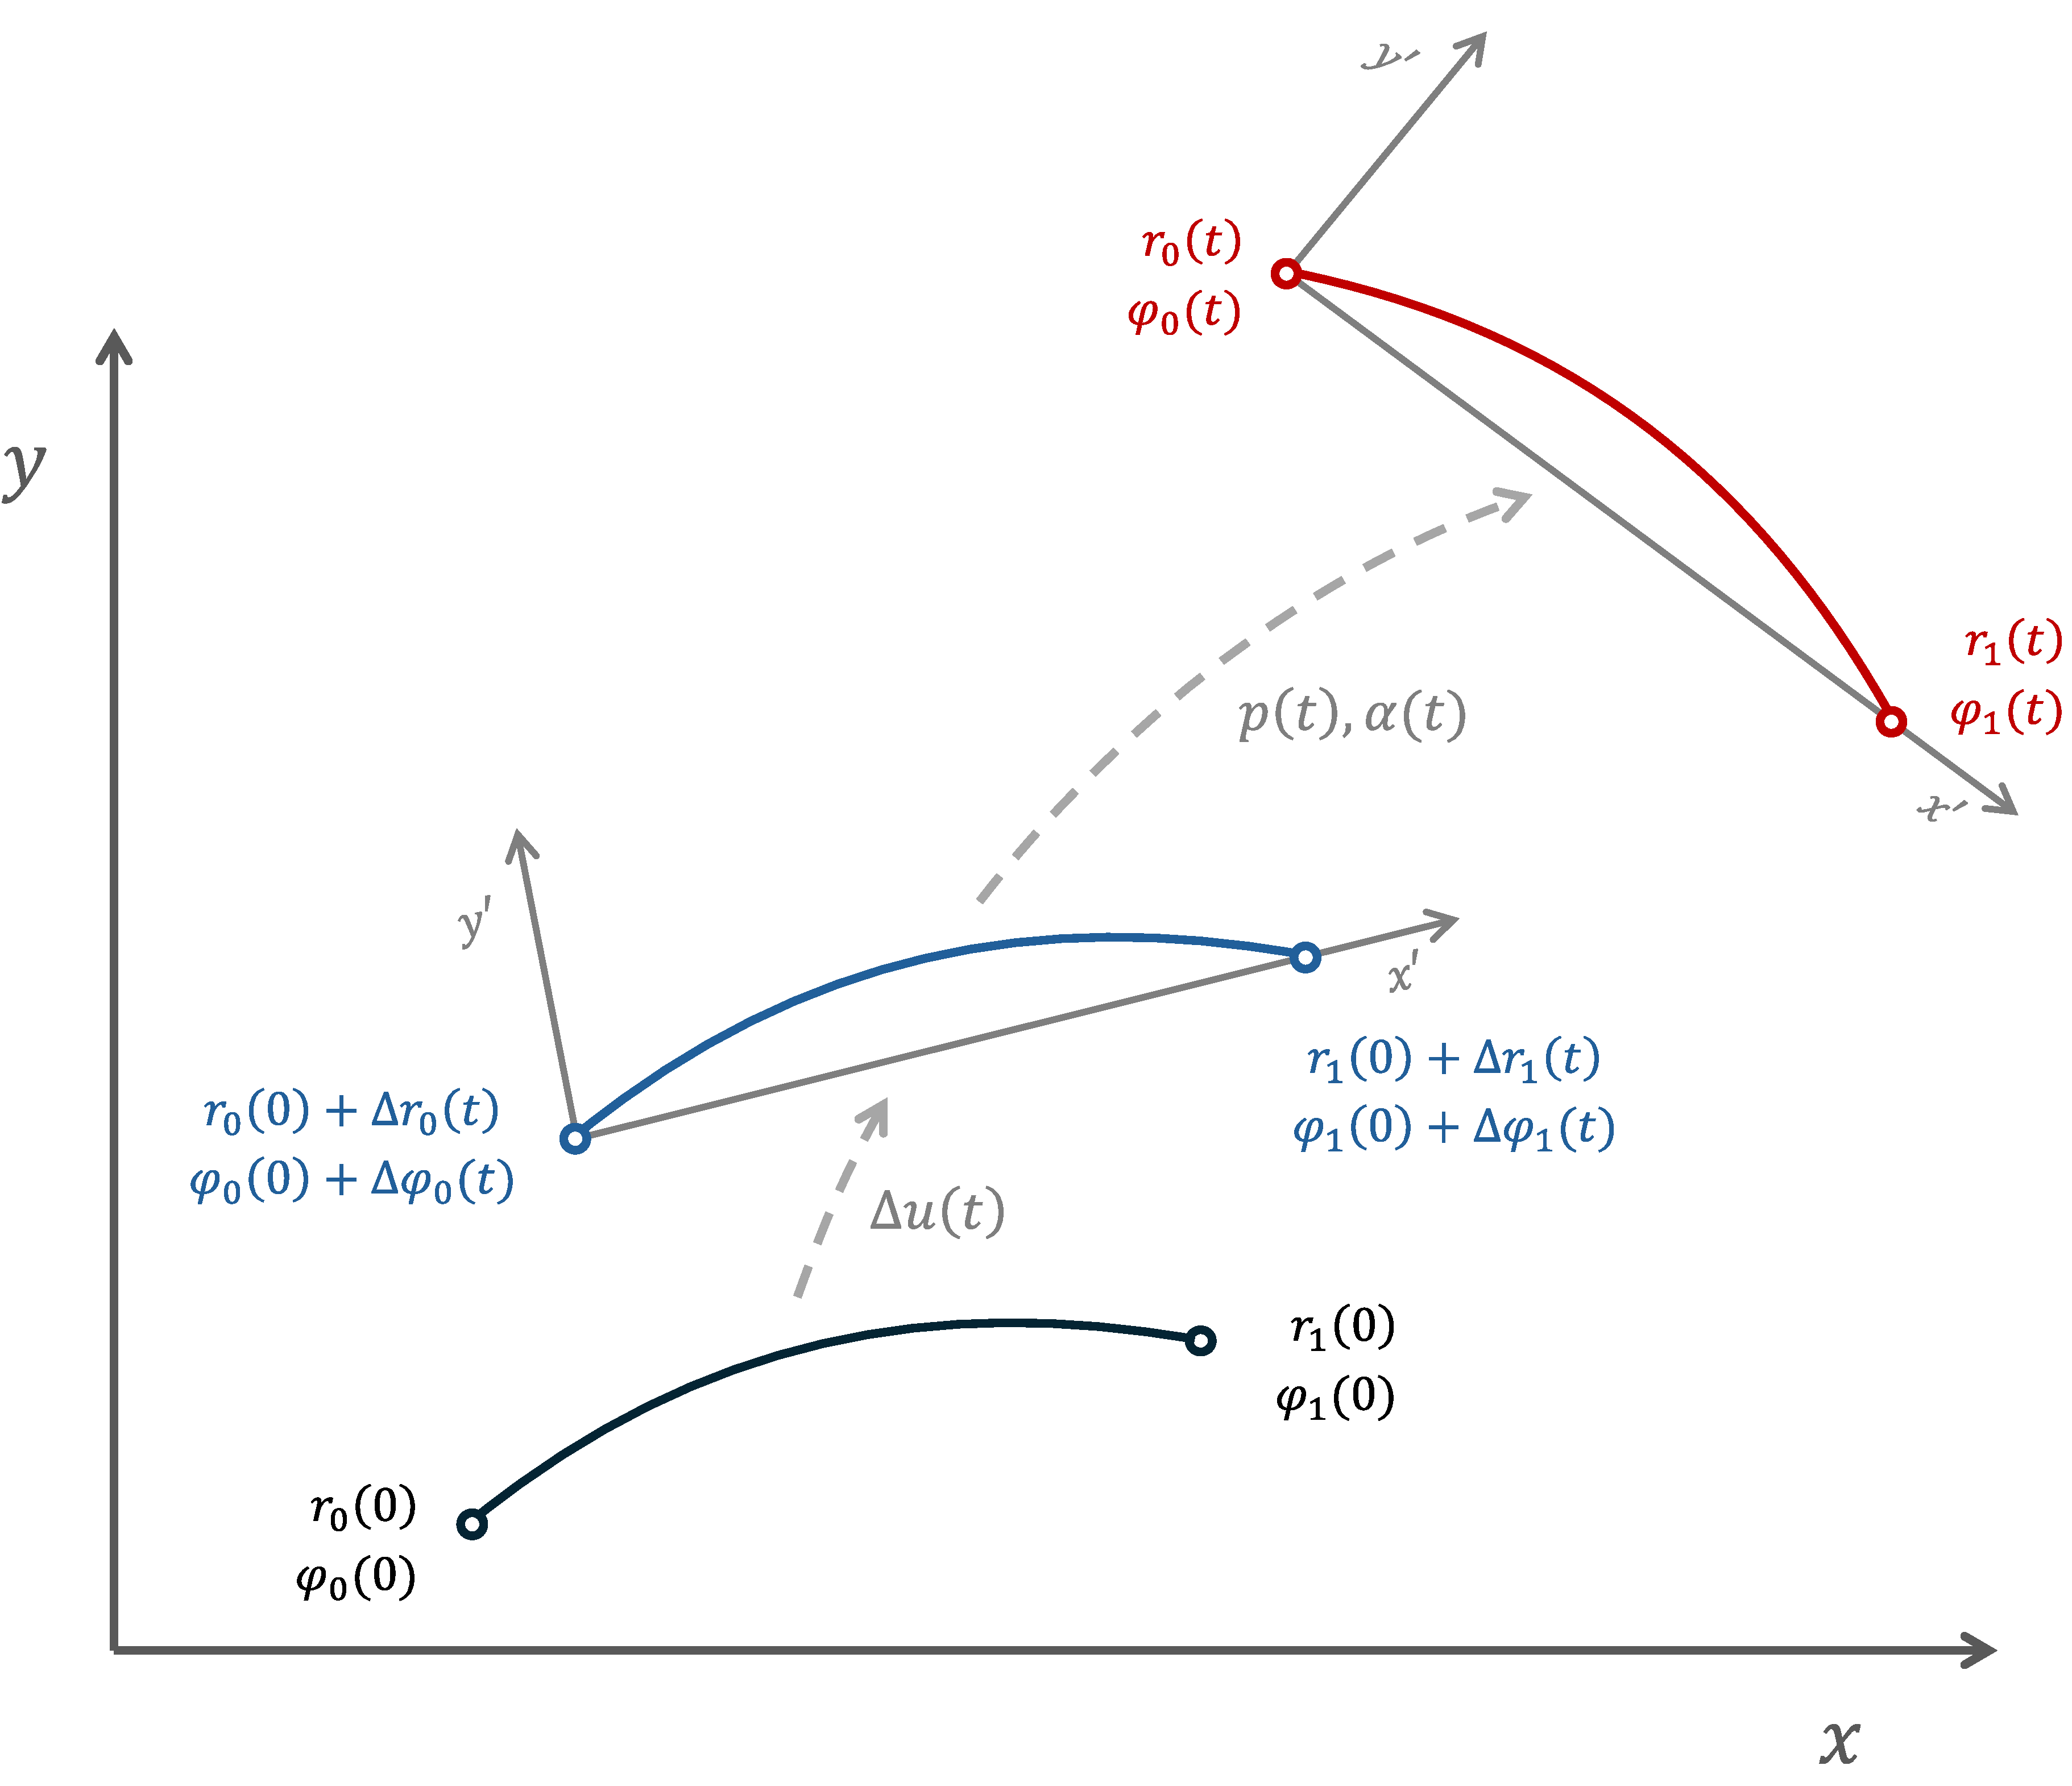
\includegraphics[width=0.8\textwidth]{figures/elements/beam-element-corotational.pdf}
\caption{Initial state (black), elastic deformation (blue) and rigid body motion (red) of the beam element}
\label{fig:beam-element-corotatrional}
\end{figure}

Extracting the rigid body motion by using a pinned reference frame:

\begin{align}
p(t) &= r_{0}(t) - r_{0}(0) - \Delta r_0(t) \\
\alpha(t) &= \angle\left(r_1(t) - r_0(t)\right) - \angle\left(r_1(0) + \Delta r_1(0) - r_0(0) - \Delta r_0(t)\right)
\end{align}

Kinematic relations:

\begin{align}
r_0(t) &= r_0(0) + \Delta r_0(t) + p(t) = r_0(t) \\
\varphi_0(t) &= \varphi_0(0) + \Delta\varphi_0(t) + \alpha(t) \\
\notag \\
r_1(t) &= r_0(t) + \lVert r_1(0) - r_0(0) + \Delta r_1(t) - \Delta r_0(t) \rVert\boldsymbol{e}_x(t) \\
\varphi_1(t) &= \varphi_1(0) + \Delta\varphi_1(t) + \alpha(t)
\end{align}

\newpage
\subsection{Mass Matrix}

As already mentioned previously \textcolor{red}{TODO: Mention}, mass matrices that are consistent with the corotational formulation tend to be fairly complicated.
For efficiency reasons, however, we would ideally want a mass matrix that is constant and diagonal, even if it's just an approximation.
That's why we derive the mass matrix in way that in't consisent with the way the elastic forces were derived, but leads to a result that has these properties.

Let's start with some general considerations before we introduce any approximations.
Let the function $\boldsymbol{p}(x,\,y,\,z)$ describt the position of the material point $(x,\,y,\,z)$ in the deformed state of the element in cartesian coordinates.
With the density $\rho$ that may vary over the element, we can express the virtual work of the inertia forces of the element as
%
\begin{align}
\delta W_{M} &= \int_{V} \delta\boldsymbol{p}^\intercal\rho\,\ddot{\boldsymbol{p}}\,dV = \int_{V} \rho\left(\frac{\partial\boldsymbol{p}}{\partial\boldsymbol{u}}\delta\boldsymbol{u}\right)^\intercal\left(\frac{\partial\boldsymbol{p}}{\partial\boldsymbol{u}}\ddot{\boldsymbol{u}}\right)\,dV = \delta\boldsymbol{u}^\intercal\underbrace{\left(\int_{V} \rho\,\frac{\partial\boldsymbol{p}}{\partial\boldsymbol{u}}^\intercal\frac{\partial\boldsymbol{p}}{\partial\boldsymbol{u}}\,dV\right)}_{\boldsymbol{M}}\ddot{\boldsymbol{u}}.
\end{align}

which gives us a general expression for the mass matrix.
In order to develop this further, we have to get more explicit about our position function.
For describing the deformation field of a beam, we write $\boldsymbol{p}$ as

\begin{equation}
\boldsymbol{p}(x,\,y,\,z) = \boldsymbol{r}(x) + y\,\boldsymbol{n}(x) + z\,\boldsymbol{b}(x)
\end{equation}

where $\boldsymbol{r}(x)$ is the beam's centerline, $\boldsymbol{n}(x)$ is the beam's normal vector and $\boldsymbol{b}(x)$ is the binormal vector (pointing out of the plane).
Further expansion and simplification of the mass matrix then leads to
%
\begin{align}
\boldsymbol{M} &= \int_{V} \rho\,\frac{\partial\boldsymbol{p}}{\partial\boldsymbol{u}}^\intercal\frac{\partial\boldsymbol{p}}{\partial\boldsymbol{u}}\,dV \notag \\
&= \int_{V} \rho\,\left(\frac{\partial\boldsymbol{r}}{\partial\boldsymbol{u}} + y\,\frac{\partial\boldsymbol{n}}{\partial\boldsymbol{u}}\right)^\intercal\left(\frac{\partial\boldsymbol{r}}{\partial\boldsymbol{u}} + y\,\frac{\partial\boldsymbol{n}}{\partial\boldsymbol{u}}\right)\,dV \notag \\
&= \int_{V} \left(\rho\,\frac{\partial\boldsymbol{r}}{\partial\boldsymbol{u}}^\intercal\frac{\partial\boldsymbol{r}}{\partial\boldsymbol{u}} + \rho y\,\frac{\partial\boldsymbol{n}}{\partial\boldsymbol{u}}^\intercal\frac{\partial\boldsymbol{r}}{\partial\boldsymbol{u}} + \rho y\,\frac{\partial\boldsymbol{r}}{\partial\boldsymbol{u}}^\intercal\frac{\partial\boldsymbol{n}}{\partial\boldsymbol{u}} + \rho y^2\,\frac{\partial\boldsymbol{n}}{\partial\boldsymbol{u}}^\intercal\frac{\partial\boldsymbol{n}}{\partial\boldsymbol{u}}\right)\,dV \notag \\
&= \int_{s_1}^{s_2} \left(\rho A\,\frac{\partial\boldsymbol{r}}{\partial\boldsymbol{u}}^\intercal\frac{\partial\boldsymbol{r}}{\partial\boldsymbol{u}} + \rho S\,\left(\frac{\partial\boldsymbol{n}}{\partial\boldsymbol{u}}^\intercal\frac{\partial\boldsymbol{r}}{\partial\boldsymbol{u}} + \frac{\partial\boldsymbol{r}}{\partial\boldsymbol{u}}^\intercal\frac{\partial\boldsymbol{n}}{\partial\boldsymbol{u}}\right) + \rho I\,\frac{\partial\boldsymbol{n}}{\partial\boldsymbol{u}}^\intercal\frac{\partial\boldsymbol{n}}{\partial\boldsymbol{u}}\right)\,ds
\end{align}

In the last step, the following three integrals over the beam's cross section have been introduced:
%
\begin{align}
\rho A(s) &= \int_A \rho\,dA \\
\rho S(s) &= \int_A \rho y\,dA \\
\rho I(s) &= \int_A \rho y^2\,dA
\end{align}

The first one, $\rho A$, is the linear density of the beam axis, i.e. the mass per unit length.
Mass matrix terms associated with this factor account for the overall motion of the beam axis.
The second one, $\rho S$, is the static moment of the cross section, weighted by its density, and is related to the excentricity of the center of gravity.
If the beam axis passed through the center of gravity of the cross sections, as is often assumed, this term would be zero.
Since we deliberately did not make this assumption, we will keep those terms for now.
The final one, $\rho I$ is the second moment of inertia of the section, weighted by its density, and accounts for the rotational inertia of the section itself.

\textcolor{red}{Introduce linear shape functions here}

The only thing left to do now is to express the derivatives $\nicefrac{\partial\boldsymbol{r}}{\partial\boldsymbol{u}}$ and $\nicefrac{\partial\boldsymbol{n}}{\partial\boldsymbol{u}}$ in terms of the shape function matrices $\boldsymbol{S}_x$, $\boldsymbol{S}_y$ and $\boldsymbol{S}_\varphi$.
This is straightforward and leads to

\begin{align}
\frac{\partial\boldsymbol{r}}{\partial\boldsymbol{u}}
&=
\frac{\partial}{\partial\boldsymbol{u}}
\begin{bmatrix}
\boldsymbol{S}_x^\intercal\boldsymbol{u} \\ \boldsymbol{S}_y^\intercal\boldsymbol{u}
\end{bmatrix}
=
\begin{bmatrix}
\boldsymbol{S}_x^\intercal \\ \boldsymbol{S}_y^\intercal
\end{bmatrix}
\\
\frac{\partial\boldsymbol{n}}{\partial\boldsymbol{u}}
&=
\frac{\partial}{\partial\boldsymbol{u}}
\begin{bmatrix}
\sin(\varphi) \\ \cos(\varphi)
\end{bmatrix}
=
\begin{bmatrix}
\boldsymbol{S}_\varphi^\intercal\cos(\varphi) \\ -\boldsymbol{S}_\varphi^\intercal\sin(\varphi)
\end{bmatrix}
\end{align}

Putting everything together, the mass matrix in its exact version becomes
%
\begin{equation}
\boldsymbol{M} = \int_{s_0}^{s_3} \left(\rho A\left(\boldsymbol{S}_x\boldsymbol{S}_x^\intercal + \boldsymbol{S}_y\boldsymbol{S}_y^\intercal\right) + \rho I\boldsymbol{S}_\varphi\boldsymbol{S}_\varphi^\intercal + \rho S\left(\left(\boldsymbol{S}_\varphi\boldsymbol{S}_x^\intercal + \boldsymbol{S}_x\boldsymbol{S}_\varphi^\intercal\right)\cos(\varphi) - \left(\boldsymbol{S}_\varphi\boldsymbol{S}_y^\intercal + \boldsymbol{S}_y\boldsymbol{S}_\varphi^\intercal\right)\sin(\varphi)\right)\right)\,ds
\end{equation}

In order to obtain a constant mass matrix, we neglect the influence of the coupling term associated with $\rho S$, leaving the simplified mass matrix

\begin{equation}
\boldsymbol{M} \approx \int_{s_0}^{s_1} \left(\rho A\left(\boldsymbol{S}_x\boldsymbol{S}_x^\intercal + \boldsymbol{S}_y\boldsymbol{S}_y^\intercal\right) + \rho I\boldsymbol{S}_\varphi\boldsymbol{S}_\varphi^\intercal\right)\,ds.
\end{equation}

This is justifiable because we are not really interested in the rotary motion of the cross sections.
We have to keep the term associated with $\rho I$ however, otherwise the mass matrix would become singular.

Diagonalized result when using the nodes as integration points (Newton-Cotes formula):

\begin{equation}
\boldsymbol{M} = \frac{s_1- s_0}{2}\begin{bmatrix}
\rho A(s_0) \\
& \rho A(s_0) \\
& & \rho I(s_0) \\
& & & \rho A(s_1) \\
& & & & \rho A(s_1) \\
& & & & & \rho I(s_1) \\
\end{bmatrix}
\end{equation}

Alternatively, the mass of the element can be computed exactly and distributed to the nodes such that the first node carries the mass of the first half of the element and the second node carries the second half.


\begin{align}
m_{0} &= \int_{s_0}^{s_m} \rho A(s)\,ds, \quad m_{1} = \int_{s_m}^{s_1} \rho A(s)\,ds \\
J_{0} &= \frac{1}{2}(s_1- s_0)\rho I(s_0), \quad J_{1} = \frac{1}{2}(s_1- s_0)\rho I(s_1)
\end{align}

\begin{equation}
\boldsymbol{M} = \begin{bmatrix}
m_0 \\
& m_0 \\
& & J_0 \\
& & & m_1 \\
& & & & m_1 \\
& & & & & J_1 \\
\end{bmatrix}
\end{equation}

\newpage
\subsection{Cross section properties}

Normal force:

\begin{align}
N(s) &= \int_A \sigma_{xx}\,dA = \int_A E\varepsilon_{xx}\,dA = \int_A E(\varepsilon - \kappa y) \notag \\
&= \left(\int_A E\,dA\right)\,\varepsilon + \left(-\int_A Ey\,dA\right)\,\kappa \notag \\
\notag \\
&= C_{\varepsilon\varepsilon}\varepsilon + C_{\varepsilon\kappa}\kappa
\end{align}

Bending moment:

\begin{align}
M(s) &= -\int_A \sigma_{xx}y\,dA = -\int_A E(\varepsilon y - \kappa y^2)\,dA \notag \\
&= \left(\int_A Ey^2\,dA\right)\,\kappa + \left(-\int_A Ey\,dA\right)\,\varepsilon \notag \\
\notag \\
&= C_{\kappa\kappa}\kappa + C_{\varepsilon\kappa}\varepsilon
\end{align}

Shear force, with $s^*$ being the actual arc length in the deformed state, probably...

\begin{equation}
Q(s) = \frac{dM}{ds^*} = \frac{dM}{ds}\frac{ds}{ds^*}
\end{equation}

\newpage
\subsection{Cross Sections (Old)}

The following derivations have been adapted from~\cite{bib:tm2} and~\cite{bib:wiki-sandwich}. Consider the laminated cross section shown in figure~\ref{fig:composite-sections-1}.
It is symmetric with respect to the~$y$-axis, bends/rotates around the~$z$-axis and consists of a number of rectangular layers. Each layer has its own density~$\rho_i$ and elastic modulus~$E_i$.
The geometry of the layers is given by their width~$w_i$, height~$h_i$ and center position~$y_i$.

\begin{figure}[h]
\centering
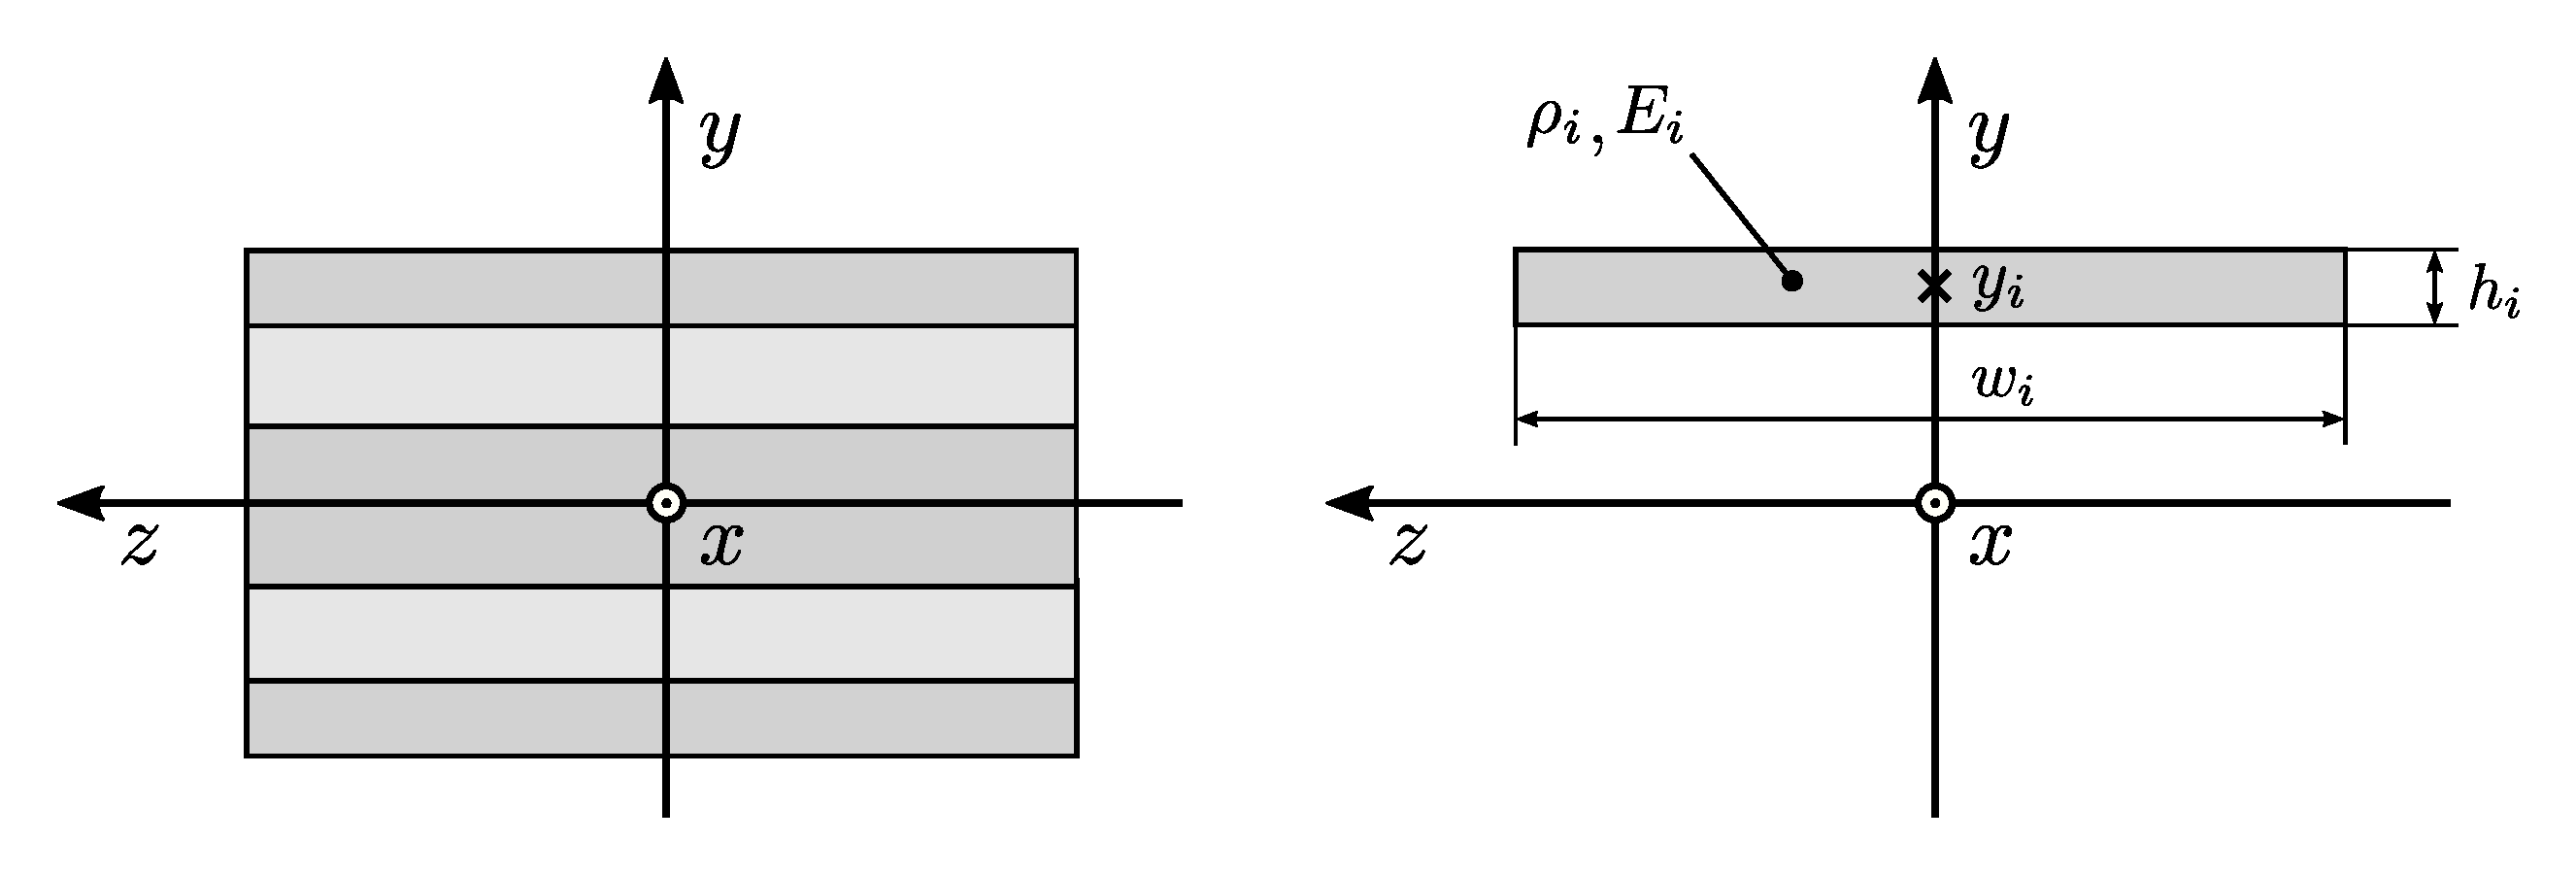
\includegraphics[width=0.9\textwidth]{figures/elements/composite-sections-1}
\caption{Composite cross section and single layer}
\label{fig:composite-sections-1}
\end{figure}

In Euler-Bernoulli beam theory the cross sections are assumed to stay flat and perpendicular to the beam axis during deformation.
We assume this to be true for our laminated cross section as well.
The distribution of longitudinal strain over the section is therefore given by the continuous function

\begin{equation}
\overline{\varepsilon}(y) = \varepsilon - \kappa\,y,
\end{equation}

where~$\varepsilon$ is the strain of the beam's centerline in $x$-direction and $\kappa$ its curvature around the $z$-axis.
The stress distribution however is not necessarily continuous, because each layer can have a different elastic modulus.
The stress within a layer is given by hooke's law as

\begin{equation}
\sigma_i(y) = E_i\cdot\overline{\varepsilon}(y),\quad y \in [y_i - \frac{h_i}{2},\,y_i + \frac{h_i}{2}].\label{eq:beam-stress-distribution}
\end{equation}

In order to determine the elastic constants in the constitutive equation~(\ref{eq:beam-constitutive}) we calculate the normal force~$N$ and bending moment~$M$ acting on the cross section by integrating the stresses~(\ref{eq:beam-stress-distribution}) over the section's area,

\begin{align}
N &= \int_A \sigma\,\mathrm{d}A = \sum_i\int_{A_i}\sigma_i\,\mathrm{d}A_i,\notag\\
&= \sum_i\int_{A_i}E_i\,\overline{\varepsilon}(y)\,\mathrm{d}A_i = \sum_i E_i \int_{A_i}(\varepsilon - \kappa\,y)\,\mathrm{d}A_i,\notag\\
&= \left(\sum_i E_i\int_{A_i}\mathrm{d}A_i\right)\varepsilon - \left(\sum_i E_i\int_{A_i}y\,\mathrm{d}A_i\right)\kappa,\notag\\
&=
\underbrace{
\left(\sum_i E_i\,A_i\right)
}_{C_{\varepsilon\varepsilon}}
\varepsilon
\underbrace{
- \left(\sum_i E_i\,A_i\,y_i\right)
}_{C_{\varepsilon\kappa}}
\kappa.\label{eq:elements:beam:constitutive_1}
\end{align}

The same can be done for the bending moment,

\begin{align}
M &= -\int_A y\,\sigma\,\mathrm{d}A = -\sum_i\int_{A_i}y\,\sigma_i\,\mathrm{d}A_i,\notag\\
&= -\sum_i\int_{A_i}y\,E_i\,(\varepsilon - \kappa\,y)\,\mathrm{d}A = -\sum_i\int_{A_i}(E_i\,\varepsilon\,y - E_i\,\kappa\,y^2)\,\mathrm{d}A,\notag\\
&= -\left(\sum_i E_i\int_{A_i}y\,dA_{i}\right)\varepsilon + \left(\sum_i E_i\int_{A_i}y^2\,dA_i\right)\kappa,\notag\\
&=
\underbrace{
-\left(\sum_i E_i\,A_i\,y_i\right)
}_{C_{\varepsilon\kappa}}
\varepsilon +
\underbrace{
\left(\sum_i E_i\,I_{i}\right)
}_{C_{\kappa\kappa}}
\kappa.\label{eq:elements:beam:constitutive_2}
\end{align}

The elastic constants describing the relationship between forces and deformation for the laminated cross section are therefore

\begin{align}
C_{\varepsilon\varepsilon} = \sum_i E_i\,A_i,\quad
C_{\kappa\kappa} = \sum_i E_i\,I_{i},\quad
C_{\varepsilon\kappa} = -\sum_i E_i\,A_i\,y_i.
\end{align}

In the case of the rectangular layers shown above, area~$A_i$ and second moment of inertia~$I_i$ evaluate to

\begin{align}
A_i &= w_i\,h_i,\\
I_i &= A_i\left(\frac{h_i^2}{12} + y_i^2\right).
\end{align}

Later we're also going to need the linear density (mass per unit length) of the laminated beam. It can be calculated by summing the the densities of the individual layers,

\begin{equation}
\overline{\rho A} = \sum_i \rho_i\,A_i.\label{eq:beam-linear-density}
\end{equation}

Pretty straightforward, compared to the other terms.
Overall, the stiffness relatio of the cross section is therefore

\begin{equation}
\begin{bmatrix}
N(s) \\ M(s)
\end{bmatrix}
=
\begin{bmatrix}
C_{ee}(s) & C_{ek}(s) \\
C_{ek}(s) & C_{kk}(s)
\end{bmatrix}
\cdot
\begin{bmatrix}
\varepsilon(s) \\ \kappa(s)
\end{bmatrix}
\end{equation}

Even though there is no shear deformation in Euler-Bernoulli beam theory, the total shear force~$Q(s)$ on the section can still be computed from static considerations as the first derivative~$M'(s)$ of the bending moment,

\begin{equation}
Q(s) = C_{kk}'(s)\,\kappa(s) + C_{ek}'(s)\,\varepsilon(s) + C_{kk}(s)\,\kappa'(s) + C_{ek}(s)\,\varepsilon'(s)
\end{equation}

\newpage
\section{String Element}

A bar only transfers forces in longitudinal direction, it has no bending stiffness. Figure~\ref{fig:bar-element-1} shows a bar with an initial length of~$l$ that is subjected to a normal force~$N$ which causes it to elongate by~$\Delta l$.

\begin{figure}[h]
\centering
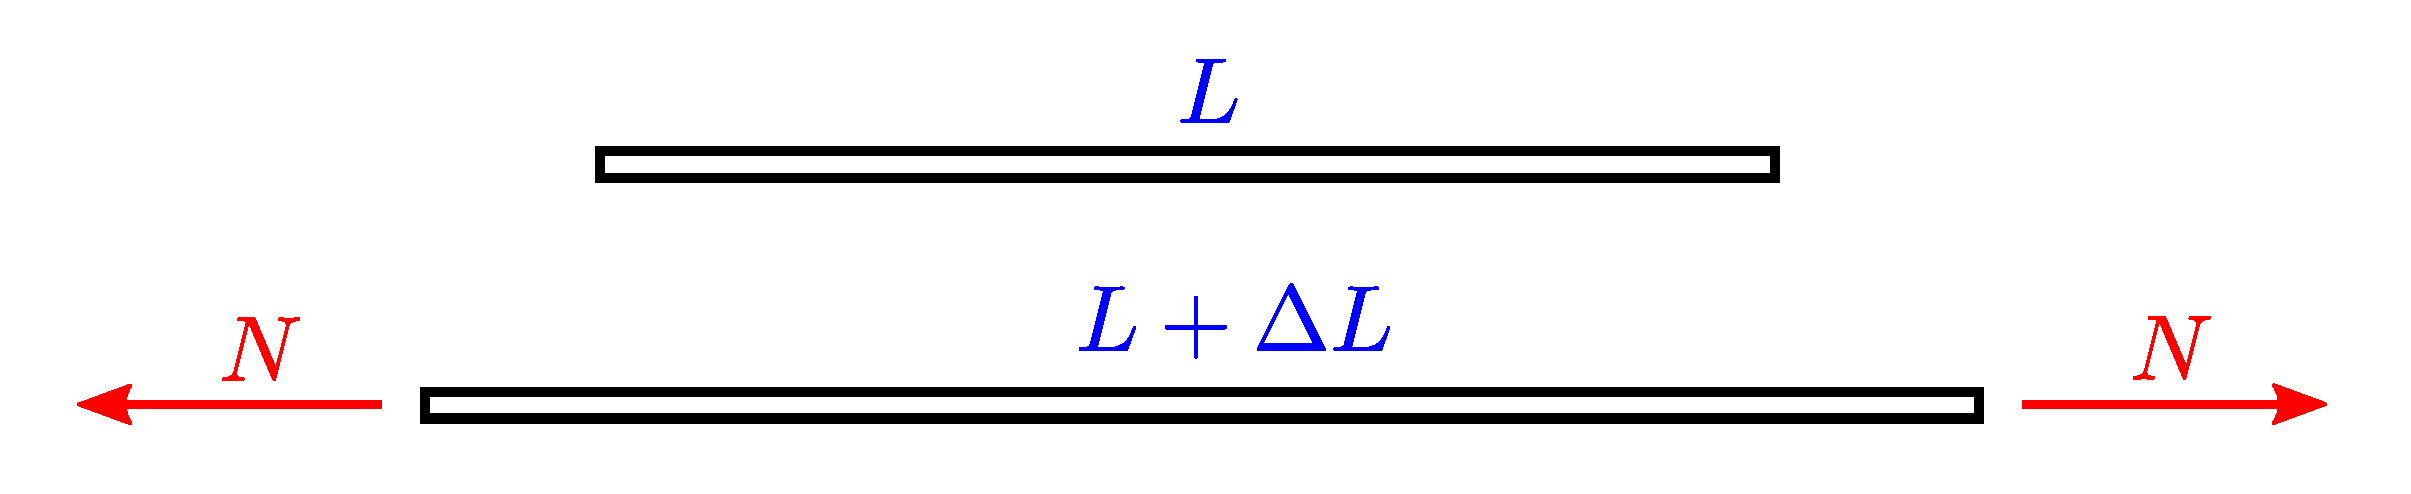
\includegraphics[width=0.75\textwidth]{figures/elements/bar-element-1}
\caption{Elongation of a bar under load}
\label{fig:bar-element-1}
\end{figure}

In order to simulate the damping properties of the string, a viscoelastic material model of the form

\begin{equation}
\sigma = E\,\varepsilon + \eta\,\dot{\varepsilon}
\end{equation}

is chosen. Here $E$ is the elastic modulus and $\eta$ the viscosity of the material. This model is called the Kelvin-Voigt model and combines linear elastic and linear viscous behaviour. The normal force in the bar given a constant cross section area $A$ is therefore

\begin{align}
N &= \sigma A \notag \\
&= EA\,\varepsilon + \eta A\,\dot{\varepsilon} \notag \\
&= \frac{EA}{l}\,\Delta l + \frac{\eta A}{l}\,\Delta \dot{l} \\
&= k\,\Delta l + d\,\Delta \dot{l}.\label{eq:bar-constitutive}
\end{align}

The product~$EA$ is also called the longitudinal stiffness.
By setting~$\varepsilon = \frac{\Delta l}{l}$ it was implicitly assumed that the strain is constant over the length of the element.
The resulting normal force (\ref{eq:bar-constitutive}) has the same form as a linear spring with stiffness~$k = \frac{EA}{l}$ and damping~$d = \frac{\eta A}{l}$.

The model for the string is an idealized spring of initial length $l_{0}$ and with constant cross section properties, given by the linear mass $\rho A$, stiffness $EA$ and damping $\eta A$.

As shown in figure \ref{fig:elements:string-element}, the current shape of the string is defined by its starting- and endpoint as well as the surface points of the limb that it contacts inbetween.
\textcolor{red}{Explain: No internal dynamics in the string, different from the old string model.}

\begin{figure}[h]
\centering
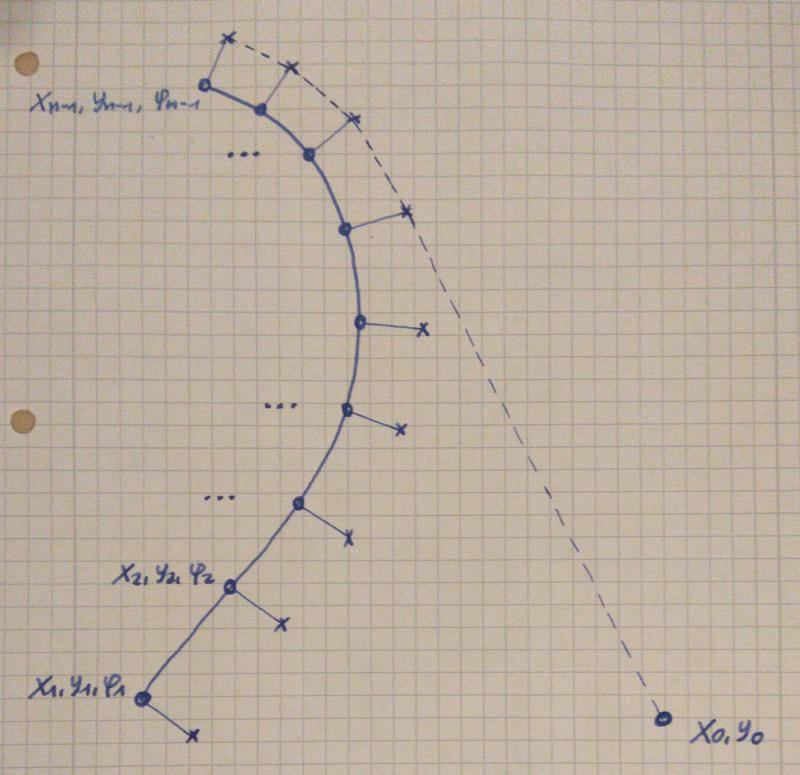
\includegraphics[width=0.5\linewidth]{figures/elements/string-element-new.jpg}
\caption{Contact interface between limb and string}
\label{fig:elements:string-element}
\end{figure}

The displacement vector $\boldsymbol{u}$ describing the string's configuration therefore has to include the starting point $x_{0}, y_{0}$ at the string center as well as the $n$ limb nodes $x_{i},\,y_{i},\,\varphi_{i}$ with $i = 1\,\ldots\,n-1$, the last of which also defines the endpoint of the string at the limb tip.
\textcolor{red}{Explain: $n$ does not have to be the whole number of nodes, can be just a subset where the string is considered likely to contact.}

\begin{equation}
\boldsymbol{u} = \begin{bmatrix}
x_{0}, & y_{0}, & x_{1}, & y_{1}, & \varphi_{1}, & \cdots & x_{n-1}, & y_{n-1}, & \varphi_{n-1}
\end{bmatrix}^\intercal
\end{equation}

The first step in evaluating the generalized forces of this element is to determine which of the limb nodes make contact with the string.
First of all, as can be seen in figure \ref{fig:elements:string-element}, the limb nodes are not the points where the string makes physical contact.
The actual contact points at the belly surface of the limb are given by

\begin{align}
\bar{x}_{0} &= x_{0}, \quad \bar{x}_{i} = x_{i} - d_{i}\sin(\varphi_{i}) \\
\bar{y}_{0} &= y_{0}, \quad \bar{y}_{i} = y_{i} + d_{i}\cos(\varphi_{i})
\end{align}

where $d_{i}$ are the perpendicular distances from the limb centerline to the surface of the limb as defined by the limb's cross section geometry.
The task of finding the contact points is then equivalent to finding the convex envelope of the points $\{x_{0},\,y_{0},\,\bar{x}_{1},\,\bar{y}_{1},\,\ldots,\,\bar{x}_{n-1},\,\bar{y}_{n-1}\}$.

\textcolor{red}{TODO: Describe algorithm for the convex envelope}

Having found the contact points we now know the exact geometrical configuration of the string and can begin formulating the internal forces for the element.
Let's denote all points that are part of the convex envelope with the index $k$.
The length between two surface points $i$ and $j$ is given by

\begin{equation}
l_{ij} = \sqrt{(\bar{x}_j - \bar{x}_i)^2 + (\bar{y}_j - \bar{y}_i)^2}
\end{equation}

The total length of the string is the sum of all line segments of the convex envelope,

\begin{equation}
l(\boldsymbol{u}) = \sum_{k} L_{k-1,k}.
\end{equation}

We use the visco-elastic Kelvin-Voigt material model to relate the stress in the string to the strain $\varepsilon$ and the strain rate $\dot{\varepsilon}$,

\begin{equation}
\sigma = E\,\varepsilon + \eta\,\dot{\varepsilon}.
\end{equation}

We further assume that the strain is constant over the whole length of the string.
This effectively disregards any internal dynamics within the string and assumes that it is always in static equilibrium.
The strain and strain rate can then be expressed in terms of the overall length $l$ as

\begin{equation}
\varepsilon = \frac{l(\boldsymbol{u}) - l_{0}}{l_{0}}, \quad \dot{\varepsilon} = \frac{1}{l_{0}}\frac{\partial l}{\partial \boldsymbol{u}}\dot{\boldsymbol{u}}
\end{equation}

Virtual work of the internal forces:

\begin{align}
\delta W_{I} &= \int_{V} \sigma\,\delta\varepsilon\,dV = \int_{0}^{l_{0}}\int_{A} \sigma\,\delta\varepsilon\,dA\,ds = \left(EA\,\varepsilon + \eta A\,\dot{\varepsilon}\right)l_{0}\frac{\partial\varepsilon}{\partial\boldsymbol{u}}\delta\boldsymbol{u}
\end{align}

And therefore the internal forces

\begin{equation}
\boldsymbol{Q}(\boldsymbol{u},\,\dot{\boldsymbol{u}}) = \left(EA\varepsilon + \eta A\dot{\varepsilon}\right)l_{0}\frac{\partial\varepsilon}{\partial\boldsymbol{u}} = \underbrace{\left(k(l - l_{0}) + d\dot{l}\right)}_{N(\boldsymbol{u},\,\dot{\boldsymbol{u}})}\frac{\partial l}{\partial\boldsymbol{u}}
\end{equation}

where $k = \frac{EA}{l_{0}}$ is the stiffness of the string and $d = \frac{\eta A}{l_{0}}$ is the damping and $N$ the normal force along the string.
The tangent stiffness matrix is derived as

\begin{align}
\boldsymbol{K} = \frac{\partial\boldsymbol{Q}}{\partial\boldsymbol{u}} &= \left(k\frac{\partial l}{\partial\boldsymbol{u}}^\intercal + d\frac{\partial\dot{l}}{\partial\boldsymbol{u}}^\intercal\right)\frac{\partial l}{\partial\boldsymbol{u}} + \left(k(l - l_{0}) + d\dot{l}\right)\frac{\partial^2 l}{\partial\boldsymbol{u}^2} \notag \\
&= \left(k\frac{\partial l}{\partial\boldsymbol{u}}^\intercal + d\dot{\boldsymbol{u}}^\intercal\frac{\partial^2 l}{\partial\boldsymbol{u}^2}\right)\frac{\partial l}{\partial\boldsymbol{u}} + \left(k(l - l_{0}) + d\dot{l}\right)\frac{\partial^2 l}{\partial\boldsymbol{u}^2} \\
\notag \\
\boldsymbol{D} = \frac{\partial\boldsymbol{Q}}{\partial\dot{\boldsymbol{u}}} &= d\frac{\partial\dot{l}}{\partial\dot{\boldsymbol{u}}}^\intercal\frac{\partial l}{\partial\boldsymbol{u}} = d\,\frac{\partial l}{\partial\boldsymbol{u}}^\intercal\frac{\partial l}{\partial\boldsymbol{u}}
\end{align}

We make no attempt at deriving a mass matrix for this element, instead we keep it massless.
The total mass $\rho A l_{0}$ of the string is instead divided between the point mass at the string center and the point mass at the limb tip of the bow model by $\nicefrac{1}{3}$ and $\nicefrac{2}{3}$, respectively.
These fractions come from symmetry considerations: Actually, when considering the whole bow, the string has a length of $2l_{0}$ and therefore a mass of $2\rho A l_{0}$.
This mass is then evenly divided between three points: $\nicefrac{1}{3}$, i.e. $\nicefrac{2}{3}\,\rho A l_{0}$ at the upper limb tip, $\nicefrac{1}{3}$ the lower limb tip and $\nicefrac{1}{3}$ at the string center.
When going back to the symmetric half-model of the bow, the center mass gets split in half, leading to $\nicefrac{1}{3}\,\rho A l_{0}$ at the string center and $\nicefrac{2}{3}\,\rho A l_{0}$ at the limb tip.
The same modellinig of the string's mass was also used by Kooi \cite{bib:kooi81}.


The last remaining task is to compute the required derivatives $\partial l/\partial \boldsymbol{u}$ and $\partial^2 l/\partial \boldsymbol{u}^2$ of the length with respect to the displacement vector.
Since the total length $l$ is a sum of partial lenbgths $l_{ij}$ between the contact points, we can compute the derivatives of the partial lengths with respect to their adjacent nodes and assemble the full derivative as

\begin{equation}
\renewcommand\arraystretch{1.5}
\frac{\partial l}{\partial \boldsymbol{u}} = \sum_{k} \frac{\partial l_{k-1,k}}{\partial \boldsymbol{u}} =
\begin{bmatrix}
\frac{\partial l_{01}}{\partial x_{0}} \\
\frac{\partial l_{01}}{\partial y_{0}} \\
\frac{\partial l_{01}}{\partial \varphi_{0}} \\
\frac{\partial l_{01}}{\partial x_{1}} \\
\frac{\partial l_{01}}{\partial y_{1}} \\
\frac{\partial l_{01}}{\partial \varphi_{1}} \\
0 \\
0 \\
0 \\
0 \\
0 \\
0 \\
\vdots
\end{bmatrix}
+
\begin{bmatrix}
0 \\
0 \\
0 \\
\frac{\partial l_{12}}{\partial x_{1}} \\
\frac{\partial l_{12}}{\partial y_{1}} \\
\frac{\partial l_{12}}{\partial \varphi_{1}} \\
\frac{\partial l_{12}}{\partial x_{2}} \\
\frac{\partial l_{12}}{\partial y_{2}} \\
\frac{\partial l_{12}}{\partial \varphi_{2}} \\
0 \\
0 \\
0 \\
\vdots
\end{bmatrix}
+
\begin{bmatrix}
0 \\
0 \\
0 \\
0 \\
0 \\
0 \\
\frac{\partial l_{23}}{\partial x_{2}} \\
\frac{\partial l_{23}}{\partial y_{2}} \\
\frac{\partial l_{23}}{\partial \varphi_{2}} \\
\frac{\partial l_{23}}{\partial x_{3}} \\
\frac{\partial l_{23}}{\partial y_{3}} \\
\frac{\partial l_{23}}{\partial \varphi_{3}} \\
\vdots
\end{bmatrix}
+
\cdots
\end{equation}

Analogous for the second derivative $\partial^2 l/\partial \boldsymbol{u}^2$, which results in a block-diagonal structure of overlapping $6 \times 6$ blocks.

First derivatives of $l_{ij}$ with respect to the positions and rotations of nodes $i$ and $j$:

% https://www.wolframalpha.com/input?i=derive+sqrt%28%28x1+-+x0%29%5E2+%2B+%28y1+-+y0%29%5E2%29+wrt+x0
% https://www.wolframalpha.com/input?i=derive+sqrt%28%28x1+-+x0%29%5E2+%2B+%28y1+-+y0%29%5E2%29+wrt+y0
% https://www.wolframalpha.com/input?i=derive+sqrt%28%28x1+-+x0%29%5E2+%2B+%28y1+-+y0%29%5E2%29+wrt+x1
% https://www.wolframalpha.com/input?i=derive+sqrt%28%28x1+-+x0%29%5E2+%2B+%28y1+-+y0%29%5E2%29+wrt+y1

\begin{align}
\frac{\partial L_{ij}}{\partial x_i} &= \frac{x_i - x_j}{L_{i,j}} , & \frac{\partial L_{ij}}{\partial y_i} &= \frac{y_i - y_j}{L_{i,j}}, & \frac{\partial L_{ij}}{\partial \varphi_i} &= -d_{i}\left(\frac{\partial L_{ij}}{\partial x_i}\cos(\varphi_i) + \frac{\partial L_{ij}}{\partial y_i}\sin(\varphi_i)\right) \\
\frac{\partial L_{ij}}{\partial x_j} &= -\frac{\partial L_{i,j}}{\partial x_i}, & \frac{\partial L_{ij}}{\partial y_j} &= -\frac{\partial L_{i,j}}{\partial y_i}, & \frac{\partial L_{ij}}{\partial \varphi_j} &= -d_{j}\left(\frac{\partial L_{ij}}{\partial x_j}\cos(\varphi_j) + \frac{\partial L_{ij}}{\partial y_j}\sin(\varphi_j)\right)
\end{align}

Second derivatives (omitting symmetric ones since $\frac{\partial l}{\partial a \partial b} = \frac{\partial l}{\partial b \partial a}$):

% https://www.wolframalpha.com/input?i2d=true&i=Partial%5B%5C%2840%29Sqrt%5BPower%5B%5C%2840%29x1+-+x0%5C%2841%29%2C2%5D%2BPower%5B%5C%2840%29y1+-+y0%5C%2841%29%2C2%5D%5D%5C%2841%29%2Cx0%2Cx0%5D

\begin{align}
\frac{\partial L_{ij}}{\partial x_i \partial x_i} &= \frac{(y_j - y_i)^2}{L_{ij}^3} \\
\frac{\partial L_{ij}}{\partial x_i \partial y_i} &= -\frac{(x_j - x_i)(y_j - y_i)}{L_{ij}^3} \\
\frac{\partial L_{ij}}{\partial x_i \partial x_j} &= -\frac{\partial L_{ij}}{\partial x_i \partial x_i} \\
\frac{\partial L_{ij}}{\partial x_i \partial y_j} &= -\frac{\partial L_{ij}}{\partial x_i \partial y_i} \\
\notag \\
\frac{\partial L_{ij}}{\partial y_i \partial y_i} &= \frac{(x_j - x_i)^2}{L_{ij}^3} \\
\frac{\partial L_{ij}}{\partial y_i \partial x_j} &= -\frac{\partial L_{ij}}{\partial x_i \partial y_i} \\
\frac{\partial L_{ij}}{\partial y_i \partial y_j} &= -\frac{\partial L_{ij}}{\partial y_i \partial y_i} \\
\notag \\
\frac{\partial L_{ij}}{\partial x_j \partial x_j} &= \frac{\partial L_{ij}}{\partial x_i \partial x_i} \\
\frac{\partial L_{ij}}{\partial x_j \partial y_j} &= \frac{\partial L_{ij}}{\partial x_i \partial y_i} \\
\notag \\
\frac{\partial L_{ij}}{\partial y_j \partial y_j} &= \frac{\partial L_{ij}}{\partial y_i \partial y_i}
\end{align}

\newpage
Angles:

Combination i, i:

\begin{align}
\frac{\partial^2 L_{ij}}{\partial x_{i} \partial \varphi_{j}} &= -d_{i}\left( \frac{\partial^2 L_{ij}}{\partial x_{i} \partial x_{i}}\cos(\varphi_{i}) + \frac{\partial^2 L_{ij}}{\partial x_{i} \partial y_{i}}\sin(\varphi_{i})\right) \\
\frac{\partial^2 L_{ij}}{\partial y_{i} \partial \varphi_{i}} &= -d_{i}\left( \frac{\partial^2 L_{ij}}{\partial y_{i} \partial y_{i}}\sin(\varphi_{i}) + \frac{\partial^2 L_{ij}}{\partial x_{i} \partial y_{i}}\cos(\varphi_{i})\right) \\
\frac{\partial^2 L_{ij}}{\partial \varphi_{i} \partial \varphi_{i}} &= -d_{i}\left(\left(\frac{\partial^2 L_{ij}}{\partial x_{i} \partial \varphi_{i}} + \frac{\partial L}{\partial \bar{y}_{i}}\right)\cos(\varphi_{i}) + \left(\frac{\partial^2 L_{ij}}{\partial y_{i} \partial \varphi_{i}} - \frac{\partial L}{\partial \bar{x}_{i}}\right)\sin(\varphi_{i})\right)
\end{align}

Combination j, j:

\begin{align}
\frac{\partial^2 L_{ij}}{\partial x_{j} \partial \varphi_{j}} &= -d_{j}\left( \frac{\partial^2 L_{ij}}{\partial x_{j} \partial x_{j}}\cos(\varphi_{j}) + \frac{\partial^2 L_{ij}}{\partial x_{j} \partial y_{j}}\sin(\varphi_{j})\right) \\
\frac{\partial^2 L_{ij}}{\partial y_{j} \partial \varphi_{j}} &= -d_{j}\left( \frac{\partial^2 L_{ij}}{\partial y_{j} \partial y_{j}}\sin(\varphi_{j}) + \frac{\partial^2 L_{ij}}{\partial x_{j} \partial y_{j}}\cos(\varphi_{j})\right) \\
\frac{\partial^2 L_{ij}}{\partial \varphi_{j} \partial \varphi_{j}} &= -d_{j}\left(\left(\frac{\partial^2 L_{ij}}{\partial x_{j} \partial \varphi_{j}} + \frac{\partial L}{\partial \bar{y}_{j}}\right)\cos(\varphi_{j}) + \left(\frac{\partial^2 L_{ij}}{\partial y_{j} \partial \varphi_{j}} - \frac{\partial L}{\partial \bar{x}_{j}}\right)\sin(\varphi_{j})\right)
\end{align}

Combination i, j

\begin{align}
\frac{\partial^2 L_{ij}}{\partial x_{i} \partial \varphi_{j}} &= -d_{j}\left( \frac{\partial^2 L_{ij}}{\partial x_{i} \partial x_{j}}\cos(\varphi_{j}) + \frac{\partial^2 L_{ij}}{\partial x_{i} \partial y_{j}}\sin(\varphi_{j})\right) \\
\frac{\partial^2 L_{ij}}{\partial y_{i} \partial \varphi_{j}} &= -d_{j}\left( \frac{\partial^2 L_{ij}}{\partial y_{i} \partial y_{j}}\cos(\varphi_{j}) + \frac{\partial^2 L_{ij}}{\partial y_{i} \partial x_{j}}\sin(\varphi_{j}) \right) \\
\frac{\partial^2 L_{ij}}{\partial \varphi_{i} \partial \varphi_{j}} &= -d_{i}\left( \frac{\partial^2 L_{ij}}{\partial x_{i} \partial \varphi_{j}}\cos(\varphi_{i}) + \frac{\partial^2 L_{ij}}{\partial y_{i} \partial \varphi_{j}}\sin(\varphi_{i})\right)
\end{align}

Combination j,i

\begin{align}
\frac{\partial^2 L_{ij}}{\partial x_{j} \partial \varphi_{i}} &= -d_{i}\left( \frac{\partial^2 L_{ij}}{\partial x_{i} \partial x_{j}}\cos(\varphi_{i}) + \frac{\partial^2 L_{ij}}{\partial x_{i} \partial y_{j}}\sin(\varphi_{i})\right) \\
\frac{\partial^2 L_{ij}}{\partial y_{j} \partial \varphi_{i}} &= -d_{i}\left( \frac{\partial^2 L_{ij}}{\partial x_{i} \partial y_{j}}\cos(\varphi_{i}) + \frac{\partial^2 L_{ij}}{\partial y_{i} \partial y_{j}}\sin(\varphi_{i}) \right)
\end{align}